\documentclass[10pt, a4paper]{report}
\usepackage[utf8]{inputenc}
\usepackage{eso-pic} % \AddToShipoutPicture
\usepackage{graphicx} % \includegraphics
\usepackage{listings} % \includegraphics
\usepackage{pgfplots}
\usepackage{hyperref}
\usepackage[utf8]{inputenc}
\usepackage{mdframed}
\usepackage{float}
\usepackage{amsmath}
\usepackage{flafter}
\usepackage{graphicx}
\usepackage{tikz}
\usepackage{blindtext}
\usepackage{pgfplots}
\usepackage{seqsplit}
\usepackage[cache=false]{minted}
\usepackage{listings}
\usepackage[htt]{hyphenat}
\usepackage{amsmath,amssymb,amsbsy}
\usepackage{graphicx}
\usepackage{amsmath,amssymb,amsbsy}
\usepackage{stmaryrd}
\usepackage{semantic}
\usepackage{url}
\usepackage{color}
\usepackage{flushend}
\usepackage{subfigure}
\usepackage{tikz}
\usepackage{svg}
\usepackage{pdfpages}
\usepackage{titling}
\usepackage{cleveref}
\usepackage[parfill]{parskip}
\usepackage[toc,page]{appendix}
%%% \usepackage{fontspec}
%%% \usepackage{titlesec}
%%% \setmainfont[
%%%   BoldFont={Minion Pro Bold},
%%%   ItalicFont={Minion Pro Italic},
%%%   BoldItalicFont={Minion Pro Bold Italic},
%%% ]{Linux Libertine O}
%%% \defaultfontfeatures{Mapping=tex-text,Scale=MatchLowercase}
%%% 
%%% \setmonofont{FreeMono}
%%% 
%%% \titleformat{\chapter}[display]
%%%   {\normalfont\fontsize{12}{15}\bfseries}
%%%   {\thesection}
%%%   {1em}
%%%   {}
%%% \titlelabel{\thetitle.\quad}
%%% 

\newcommand{\fshark}{{\texttt{FShark}}}
\newcommand{\fsharp}{{\texttt{F\#}}}
\newcommand{\csharp}{{\texttt{C\#}}}
\newcommand{\clang}{{\texttt{C}}}
\newcommand{\Python}{{\texttt{Python}}}
\newcommand{\fsharpexpr}{\texttt{FSharpExpr}}
\newcommand{\fsharkexpr}{\texttt{FSharkExpr}}
\newcommand{\fsharkil}{\texttt{FSharkIL}}
\newcommand{\fsharkcompiler}{\texttt{FSharkCompiler}}
\newcommand{\fsharkwrapper}{\texttt{FShark Wrapper}}

\newenvironment{longlisting}{\captionsetup{type=listing}}{}

\setminted{fontsize=\small,baselinestretch=1,frame=lines,framerule=0.3pt,linenos}
\lstset{basicstyle=\small,frame=lines,numbers=left}
\usepackage[english, science, titlepage]{ku-frontpage}

\title{FShark}
\assignment{Master's thesis}
\author{Mikkel Storgaard Knudsen}

\subtitle{Futhark programming in FSharp}
\date{Handed in: \today{}}
\advisor{Advisor: Cosmin eller Troels}
\frontpageimage{hedgehogshark_cropped.jpg}

\author{Mikkel Storgaard Knudsen}

\usepackage{tcolorbox}
\usepackage{etoolbox}
%\BeforeBeginEnvironment{minted}{\begin{tcolorbox}}%
%\AfterEndEnvironment{minted}{\end{tcolorbox}}%

% Futhark syntax highlighting setup
\usepackage{listings}
\renewcommand{\ttdefault}{pcr} % Courier instead of Computer Modern
% Fix dashes in listings (from
% https://tex.stackexchange.com/questions/33185/listings-package-changes-hyphens-to-minus-signs
% )
\makeatletter
\lst@CCPutMacro\lst@ProcessOther {"2D}{\lst@ttfamily{-{}}{-{}}}
\@empty\z@\@empty
\makeatother
\lstdefinelanguage{Futhark}
{keywords={fun,if,then,else,loop,do,map,reduce,reduceComm,filter,scan,redomap,redomapComm,transpose,reshape,iota,replicate,let,in,for,while,with,f32,int,zip,streamSeq,zipWith,unsafe,streamRed,streamMap,mapPerThread,fn,reduceKernel,concat,split,size},%
  sensitive=true,
  comment=[l]{--},
  moredelim=**[is][\color{blue}]{$}{$}
}
\lstdefinelanguage{tail}
{keywords={let,in},%
  sensitive=true,
  comment=[l]{--},
  moredelim=**[is][\color{blue}]{$}{$}
}
\lstset{
  language=Futhark,
  basicstyle=\ttfamily,
  keywordstyle=\bfseries,
  showlines=true,
  columns=fullflexible,
  keepspaces=true,
}
% for adjustwidth environment
\usepackage[strict]{changepage}

\setlength{\abovecaptionskip}{3pt plus 0pt minus 2pt} % Chosen fairly arbitrarily

% for formal definitions
\usepackage{framed}

% environment derived from framed.sty: see leftbar environment definition
\definecolor{formalshade}{rgb}{0.95,0.95,1}

\newenvironment{formal}{%
  \def\FrameCommand{%
    \hspace{1pt}%
    {\color{formalshade}\vrule width 4pt}%
    \colorbox{formalshade}%
  }%
  \MakeFramed{\advance\hsize-\width\FrameRestore}%
  \noindent\hspace{-4.55pt}% disable indenting first paragraph
  \begin{adjustwidth}{}{7pt}%
  \vspace{2pt}\vspace{2pt}%
}
{%
  \vspace{2pt}\end{adjustwidth}\endMakeFramed%
}

\newcommand{\evals}[1]{\llbracket #1 \rrbracket}
\newcommand{\evalfn}[1]{\evals{#1}_{\textrm{fn}}}
\newcommand{\evalbinop}[1]{\evals{#1}_{\textrm{binop}}}
\newcommand{\evalunop}[1]{\evals{#1}_{\textrm{unop}}}
\newcommand{\id}[1]{\emph{#1}}
\newcommand{\lit}[1]{\text{\ttfamily #1}} % literal

\definecolor{rosso}{RGB}{220,57,18}
\definecolor{giallo}{RGB}{255,153,0}
\definecolor{blu}{RGB}{102,140,217}
\definecolor{verde}{RGB}{16,150,24}
\definecolor{viola}{RGB}{153,0,153}

\makeatletter

\tikzstyle{chart}=[
    legend label/.style={font={\scriptsize},anchor=west,align=left},
    legend box/.style={rectangle, draw, minimum size=5pt},
    axis/.style={black,semithick,->},
    axis label/.style={anchor=east,font={\tiny}},
]

\tikzstyle{bar chart}=[
    chart,
    bar width/.code={
        \pgfmathparse{##1/2}
        \global\let\bar@w\pgfmathresult
    },
    bar/.style={very thick, draw=white},
    bar label/.style={font={\bf\small},anchor=north},
    bar value/.style={font={\footnotesize}},
    bar width=.75,
]

\tikzstyle{pie chart}=[
    chart,
    slice/.style={line cap=round, line join=round, very thick,draw=white},
    pie title/.style={font={\bf}},
    slice type/.style 2 args={
        ##1/.style={fill=##2},
        values of ##1/.style={}
    }
]

\pgfdeclarelayer{background}
\pgfdeclarelayer{foreground}
\pgfsetlayers{background,main,foreground}


\newcommand{\pie}[3][]{
    \begin{scope}[#1]
    \pgfmathsetmacro{\curA}{90}
    \pgfmathsetmacro{\r}{1}
    \def\c{(0,0)}
    \node[pie title] at (90:1.3) {#2};
    \foreach \v/\s in{#3}{
        \pgfmathsetmacro{\deltaA}{\v/100*360}
        \pgfmathsetmacro{\nextA}{\curA + \deltaA}
        \pgfmathsetmacro{\midA}{(\curA+\nextA)/2}

        \path[slice,\s] \c
            -- +(\curA:\r)
            arc (\curA:\nextA:\r)
            -- cycle;
        \pgfmathsetmacro{\d}{max((\deltaA * -(.5/50) + 1) , .5)}

        \begin{pgfonlayer}{foreground}
        \path \c -- node[pos=\d,pie values,values of \s]{$\v\%$} +(\midA:\r);
        \end{pgfonlayer}

        \global\let\curA\nextA
    }
    \end{scope}
}
 
\newcommand{\legend}[2][]{
    \begin{scope}[#1]
    \path
        \foreach \n/\s in {#2}
            {
                  ++(0,-10pt) node[\s,legend box] {} +(5pt,0) node[legend label] {\n}
            }
    ;
    \end{scope}
}

\begin{document}

%%%% CHAPTERS
\maketitle{}

\clearpage



\begin{abstract}
  \large{ Here is a nice abstract} \\
  prut prut

\end{abstract}








\clearpage
\tableofcontents

\chapter*{}

%%% Local Variables:
%%% mode: latex
%%% TeX-master: "../thesis"
%%% End: 
\chapter{Introduction}
Developers worldwide are, and have always been, on the lookout for increased
computing performance.
Until recently, the increased performance could easily be
achieved through advances within raw computing power, as CPU's had steadily been
doubling their number of on-chip transistors, in rough accordance to Moore's Law (citér
her).

As performance increases in single-CPU design has stalled due to the power
wall\cite{powerwall} (among other things), developers are turning to multi-core
processors instead. As the number of cores increases, so does the number of
active threads available for parallel data processing.

Modern mainstream GPUs can run tens of thousands of threads in
parallel. Modern mainstream CPUs, like the current Ryzen series by AMD, usually
support between 10 and 20 simultaneous threads.
This makes GPUs the optimal target for data-parallel programming.

GPU programming is complicated: GPU-targeting developers must not only
write the computational kernels for the GPUs, but also often manually handle the
memory allocations and -transfers between the main program and the GPU device.
Such difficulties in GPU development, compared to normal (sequential) CPU
development, severely hinders the adaption of GPU programming in general.

Even though most programming languages support GPU programming through various
libraries, there are very solutions that offers GPU programming through high
level programming \-- the users still have to write their own kernels in some
form, and likewise declare their own buffers.

Two mainstream languages which lack high level GPU programming solutions are
\csharp{} and \fsharp{}. 

It is safe to say that there exists plenty of \csharp{} and \fsharp{} projects
in the real world, which could greatly benefit from parallelizing parts of their
algorithms, but current solutions would then demand that those parts in
particular
should be rewritten at least partly as GPU code, depending on the libraries
used. Depending on someone to have non-mainstream GPU coding skills on a
conventional developer team is not feasible, so the benefits from parallelizing
are often left alone in favor of maintaining a more accessible code base.
\clearpage

Currently, there does exist plenty of high level solutions to this problem.
In particular, numerous domain specific languages exists that allows programmers
to solve their domain specific problems in a high level language, and compile it
to standalone GPU accelerated libraries or programs.

Of such DSLs we have for instance:
\begin{itemize}
\item Forma
\item Ebb
\item one more
\end{itemize}

However, DSLs such as these are always either embedded in some host language
(such as Accelerate), or compiled to standalone executable programs. Their
compilers are designed to optimize performance, but rarely to support
interoperability to any significant degree.

Projects like APLtail\cite{apltail} have shown new ways to obtain GPU-accelerated
executables and libraries from source code written in  high level language. APLtail parses
and compiles APL\footnote{more accurately a subset of the APL language} code into redistributable C or Python libraries.

In summary, the hardware for massively parallel programming is widely available.
Furthermore, solutions exists for writing efficient GPU programs in high level
languages, but these have weak interoperability support with mainstream
languages.

\section{What \fshark{} sets out to do}
This thesis takes inspiration from APLtail\cite{apltail}, and creates a solution
that lets users compile efficient GPU programs from a high level programming
language, whilst at the same time supporting a high level of interoperability
with a mainstream language.
Whereas APLtail allows integration of GPU Futhark-written computation kernels in
C- and Python programs (by means of code generation), we would like to use code generation to make Futhark-written kernels available for use in \csharp{} and \fsharp{} programs.

To show that this is feasible, we first design a \csharp{} code generator for the
Futhark compiler. This code generator must be able to generate \csharp{} source
files, that can be compiled and used either as standalone executables, or as
importable libraries in any other \csharp{} or \fsharp{} program.
MERE HER

The code generator alone should not convince anyone that we are creating GPU
kernels from a high level language, which is why we also design and implement a
compiler which takes source code written in a mainstream language, compiles it
as efficient GPU kernels, and (together with the code generator) makes the
resulting GPU program immediately operable from the mainstream language itself.  

Empirical evaluation demonstrates that this approach is feasible.
We both show that that unit tests written in a high level language can be compiled and executed
correctly as computational kernels on the GPU, just as we also take complex
benchmark programs written in a mainstream language, compile them into
computational kernels for the GPU, and use them directly in the mainstream
language afterwards.































\section*{Motivation}
\fshark{} is intended to be a way of writing and utilizing Futhark, without
actually having to write or interact with the Futhark language and compiler
itself. Besides some tooling and an \fsharp{} SOAC library, it primarily consists of the \fshark{} compiler that compiles from
\fsharp{} source code to Futhark source code, and the Futhark \csharp{}
generator, which compiles Futhark programs as either standalone \csharp{}
programs or -libraries.

As much as most developers are happy to increase performance on big
computations, it is not always an option to incorporate an extra langauge into
an already existing programming language. At this moment, using Futhark in
either a \csharp{}- or \fsharp{} project is a contrived process that usually
requires spawning a subprocess with a \texttt{futhark-opencl} C program from inside one of the .NET
projects.

In order to use Futhark natively in .NET languages, it is therefore
necessary to write a backend for Futhark in a .NET language.
For \fshark{}, I have chosen to implement this backend in \csharp{}, as the Futhark intermediate
code \texttt{ImpCode}\footnote{which stands for Imperative Code} is trivial to
translate into imperative \csharp{} statements and expressions.
Also, there are \csharp{} libraries available which supply OpenCL bindings, which are
needed to implement the necessary OpenCL constructs from \texttt{ImpCode}.

It is my belief that exporting Futhark programs as .NET executables and
-libraries will lower the barrier to Futhark usage in .NET projects
significantly, hopefully increasing the all-round number of Futhark users, and
in the long term, increasing utilization of GPU programming and making it more
widely available.

However, one could do even more than just exporting Futhark to .NET, to increase
accessibility:

As tens of thousands of programmers worldwide (CHECK NUMBER JEEEEZ) are already
writing \fsharp{} programs, and that most of \fsharp{}s functional language features can be
directly translated into equivalent Futhark features, it became worthwhile to
investigate whether it was possible to design a way for users to both write and
utilize Futhark in \fsharp{} projects, without ever actually touching the
Futhark language or compiler themselves.
Instead, users can write their data parallel \fsharp{} modules in \fshark{}, and compile these
modules into Futhark libraries automatically.

In this case, it would be possible to get Futhark speeds in \fsharp{} programs,
without doing much more than installing the Futhark compiler locally, and adding
the required \fshark{} libraries to the \fsharp{} project.

It is my belief that being able to achieve Futhark performance in regular \fsharp{}
programs almost automatically, will make it significantly easier for people to
adapt to Futhark programming.

(SOME MORE MORE SOME MORE)

\clearpage
\section*{The contributions of this thesis}
The contributions of this thesis are as follows:
\begin{enumerate}
\item The \texttt{FSharkPrelude}:\\
  The \texttt{FSharkPrelude} is a subset of the Futhark SOACs, ported to
  \fsharp{}. To write an \fshark{} program, the user is directed to limit
  himself to the SOACs in the \texttt{FSharkPrelude}. This means exchanging
  \texttt{Array.map} for \texttt{FSharkPrelude.Map}, \texttt{Array.foldBack} for
  \texttt{FSharkPrelude.foldr}, and so on.
  However, the \texttt{FSharkPrelude} carries the guarantee, that all
  \texttt{FSharkPrelude} functions works equivalently to their Futhark SOAC namesakes. 
  This prelude, together with the \fsharp{} subset chosen for \fshark{}, makes
  it possible to write \fsharp{} programs which, when translated to Futhark
  code, are equivalent to their Futhark counterparts.

\item An \fsharp{} subset translatable with \fshark{}:\\
  As \fsharp{} is not only a multi-paradigm language, but also has access to the
  entire standard .NET library, it was required to make \fshark{} support only a
  subset of \fsharp{}. This has been implemented by whitelisting only the
  \fsharp{}-to-Futhark translatable types, constructs and expressions in the \fshark{}
  compiler. Furthermore, no other module imports than \texttt{FSharkPrelude} are allowed. 
  This subset is of course documented for users.

\item The \fshark{} Compiler and Wrapper:\\
  The \fshark{} Compiler and Wrapper takes a module written in \fshark{} as
  input, converts the \fshark{} module into a compiled Futhark \csharp{} module,
  and makes it available to the \fsharp{} program, all at runtime.
  The pipeline is described in sec \ref{chapter:fsharkcompiler}

\item A \csharp{} backend for Futhark:\\
  To actually use Futhark in \csharp{} projects (and transitively \fsharp{}
  projects), it was necessary to develop and add a \csharp{} backend to
  the Futhark compiler. This backend is equivalent in functionality to
  the \texttt{C}- and the \texttt{Python} backends that are already available.

\end{enumerate}

\clearpage
\section*{Vocabulary}
Unless otherwise specified, these are the terms used in the thesis:
\begin{description}
\item[For \fshark{}]\hfill
  \begin{itemize}
  \item The \fshark{} \textit{subset} is the subset of the \fsharp{} language
    that is supported by the \fshark{} compiler.

  \item The FShark Prelude is the library of \fsharp{}-ported Futhark array
    functions and SOACs, and is included with \fshark{}.

  \item \fshark{} code is \fsharp{} code which exclusively uses the \fshark{}
    subset and FSharkPrelude.

  \item \fshark{} modules are \fsharp{} modules written entirely in \fshark{}
    code.
    
  \item \fshark{} projects are \fsharp{} projects which uses \fshark{} and
    \fshark{} modules.
    \\
  \end{itemize}

\item[For Futhark]\hfill
  \begin{itemize}

  \item Futhark code is code written in Futhark.

  \item Futhark C-, Python- or \csharp{} code refers to Futhark code that has been compiled
    into C-, Python or \csharp{} source code.

  \end{itemize}
\end{description}



\section*{Roadmap}
The main part of this thesis is split in four parts.
blaaaah


%%% Local Variables:
%%% mode: latex
%%% TeX-master: "../thesis"
%%% End:
\chapter{Background}
In this chapter we will first show two languages for GPU programming, namely
CUDA and Futhark. Then we will show \csharp{} and it's interoperability with
Futhark.
Finally, we will take a look at \fsharp{}, and how we can expect
Futhark/\fsharp{} interoperability.

\section{CUDA}
GPU programming is in principle easily available for everyone. As long as the user has access
to a GPU and a reasonable PC for developing software, it just takes a bit of effort and reading to get started with CUDA, OpenCL or similar programming.
Realistically however, it takes much more than just a little effort to start
writing one's own GPU programs. 

\subsection{A simple CUDA program}
Take for instance the function $f(x,y) = ax+y$. In figure \ref{fig:cudasaxpy} we see the
function implemented as a CUDA program. In this program, we are defining the
kernel \texttt{saxpy} itself, and also manually copying data back and forth
between the GPU.

\subsubsection{The CUDA kernel}
Line 3's \texttt{\_\_global\_\_} signifies that the following function is a CUDA kernel.
Line 4 to 10 contains the computational kernel for the GPU.
Line 4 contains the kernels name and arguments. The kernel takes as arguments
\textit{a} is a scalar constant, the pointers \textit{x} and \textit{y} are
references to floating point arrays in the GPU device memory, and \textit{n}
denotes the length of the arrays \textit{x} and \textit{y}.\\
Line 6 computes the current computational thread's global id $i$. If we compare
a parallel computational kernel with a sequential for-loop, this global id is
the iterator variable.
Line 8 performs the actual $f(x,y)$ calculation, and stores the result in the y
array, but only if the if-clause in line 7 is true.
As we have tens of thousands of threads running simultaneously on the CUDA
device, we only want to perform any array operations if we know that our current
global id is within the length of the array.
\\\\

\subsubsection{The CUDA main function}
We also need a main function to run the kernel:\\
Line 14 sets N to $1 << 20$ (or $2^{20}$).\\
Line 16 and 17 allocates memory for two arrays x and y in system memory.\\
Line 19 and 20 allocates memory for two arrays x and y on the CUDA device (the GPU.)\\
Line 22 to 25 initializes the arrays x and y with scalar values 1.0 and 2.0.\\
Line 27 and 28 copies our arrays from system memory to the corresponding arrays on
th CUDA device.\\
Line 31 executes the \texttt{saxpy} kernel.\\
Line 33 copies the result from CUDA device back to the y array in the system
memory. \\
The remaining lines frees the allocated memory, first from the CUDA device and
then from the system memory.

\begin{figure}[H]
  \centering
\begin{minted}[linenos]{cpp}
  #include <stdio.h>

__global__
void saxpy(int n, float a, float *x, float *y)
{
  int i = blockIdx.x*blockDim.x + threadIdx.x;
  if (i < n){
    y[i] = a*x[i] + y[i];
  }
}

int main(void)
{
  int N = 1<<20;
  float *x, *y, *d_x, *d_y;
  x = (float*)malloc(N*sizeof(float));
  y = (float*)malloc(N*sizeof(float));

  cudaMalloc(&d_x, N*sizeof(float)); 
  cudaMalloc(&d_y, N*sizeof(float));

  for (int i = 0; i < N; i++) {
    x[i] = 1.0f;
    y[i] = 2.0f;
  }

  cudaMemcpy(d_x, x, N*sizeof(float), cudaMemcpyHostToDevice);
  cudaMemcpy(d_y, y, N*sizeof(float), cudaMemcpyHostToDevice);

  // Perform SAXPY on 1M elements
  saxpy<<<(N+255)/256, 256>>>(N, 2.0f, d_x, d_y);

  cudaMemcpy(y, d_y, N*sizeof(float), cudaMemcpyDeviceToHost);

  cudaFree(d_x);
  cudaFree(d_y);
  free(x);
  free(y);
}
\end{minted}
  \caption{$ax + y$ in CUDA}
  \label{fig:cudasaxpy}
\end{figure}


\section{Futhark}
Whereas the CUDA program and kernel contained large amounts of memory handling
and bounds checking, a similar program written in Futhark spares us for a lot of
the manual labor above. Figure \ref{fig:futsaxpy} contains a Futhark program
that is semantically equivalent to the CUDA program, in regards to the
computational result.
\begin{figure}[H]
  \centering
\begin{lstlisting}[language=Futhark, numbers=left]
let saxpy (a : f32) (x : f32) (y : f32) : f32 =
  a*x+y

entry main =
  let N = 1<<20
  let a = 2f32
  let xs = replicate N 1f32
  let ys = replicate N 2f32
  let ys' = map2 (saxpy a) xs ys
  in ys'
  \end{lstlisting}
  \caption{$ax+y$ in Futhark}
  \label{fig:futsaxpy}
\end{figure}

Line 1 to 2 defines a function that takes three floats (\textit{a}, \textit{x}
and \textit{y}) and returns $ax+y$.  

Line 4 to 10 defines our main function.\\
In line 4 we use \texttt{entry} instead of \texttt{let} to tell the compiler
that \texttt{main} is an entry point in the compiled program. This means we can
call this function when we import the compiled program as a library, as opposed
to the function \texttt{saxpy}, which cannot be accessed as a library function.\\
Line 5 sets N to $1 << 20$ (or $2^{20}$).\\
Line 6 sets a to 2.0.\\
Line 7 uses the built-in function \texttt{replicate}\footnote{replicate has the
  type \texttt{int -> a -> []a}} to generate an N element
array of 1.0\\
Line 8 uses the built-in function \texttt{replicate} to generate an N element array of 2.0\\
Line 9 uses the built-in function \texttt{map2} to apply the curried function
(\texttt{saxpy a}) to the arrays xs and ys.

\texttt{map f xs} has the type \texttt{((a -> b) -> []a -> []b)}, and
returns the array of f applied to each element of xs.

\texttt{map2 f xs ys} is very similar, but has the type \texttt{((a -> b -> c) -> []a -> []b -> []c)}, and
applies f to the elements of xs and ys pairwise.\\
In this case, we are calling \texttt{map2} with the function \texttt{(saxpy a)},
which is just \texttt{saxpy} with the first argument $a$ already defined.

When we compare the program in figure \ref{fig:cudasaxpy} to the same program
written in Futhark (figure \ref{fig:futsaxpy}), we quickly see how Futhark's
high level declarative approach is simpler and less verbose than CUDA's.
The Futhark compiler does the heavy lifting, by parsing Fuhark source code and
generating OpenCL code and wrapping them in standalone C- or Python programs.

\section{\fsharp{}}
\fsharp{} is a high level multi-paradigm programming language in the .NET family.
\fsharp{}s syntax follows a classical functional programming style. For
instance, this means we can take (some programs) written in Futhark, and port
them to \fsharp{} in a way that very closely resembles the original Futhark
code.

Figure \ref{fig:fsharpsaxpy} shows the Futhark program from
\ref{sec:futharkintro} written in \fsharp{}.

\begin{figure}[H]
  \centering
\begin{minted}[linenos]{fsharp}
let saxpy (a : single) (x : single) (y : single) : single =
  a*x+y
  
let main =
  let n = 1<<<20
  let a = 2.0f
  let xs = array.replicate n 1.0f
  let ys = array.replicate n 2.0f
  let ys' = array.map2 (saxpy a) xs ys
  in ys'
  \end{minted}
  \caption{$ax+y$ in Futhark}
  \label{fig:fsharpsaxpy}
\end{figure}

\fsharp{} also supports object oriented programming, and has seamless
interoperability with the rest of the .NET language family. We can therefore
readily use \csharp{} libraries and classes in \fsharp{}, and vice versa.

\section*{\csharp{}}
\csharp{} 
\csharp{} 
\csharp{} 
\csharp{} 

%%% Local Variables:
%%% mode: latex
%%% TeX-master: "../thesis"
%%% End:

\chapter{Birds-Eye View:\\Architecture and Use Cases}

\section{Generating GPU accelerated libraries}
In this thesis, we are interested in making Futhark-generated GPU kernels available
in \csharp{} programs.
Currently, Futhark source code can be compiled to C and Python code.
For example, the Futhark C compiler follows the basic architecture shown in
figure \ref{fig:ccompiler}.
When we call the Futhark C compiler \texttt{futhark-c} on a Futhark source file, 
the compiler reads the source code file (and possibly imports) into a high-level
compiler representation.
As the compiler applies different passes to optimize the program, it also 
successively re-writes it using lower-level but still pure-functional 
intermediate representations (IR).  The last step in the blue box is to generate
an imperative IR, which is not subject to further Futhark optimizations.
This imperative IR is the input to various code generators, for example, 
the second box in the figure will perform a translation to the C language.
The resulting C souce file contains allows the exports of the original Futhark 
to be used in an intuitive fashion from any other C program.

The Python compilation pipeline follows a similar strategy.

\begin{figure}[H]
  \centering
  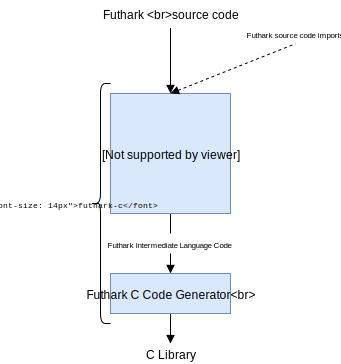
\includegraphics{chapters/figs/architecture/ccompiler.pdf}
  \caption{The Futhark-to-C compilation pipeline}
  \label{fig:ccompiler}
\end{figure}

\subsection{Using Futhark in Python}
We will now describe a use case for the Futhark-to-Python compiler:
\begin{enumerate}
\item We write a short Futhark program, which has a single entry function
    available. This program takes an array of integers, and
    adds 2 to each element in the array. The program is saved in file 
    {\tt mapPlus2.fut} and is shown below: %in figure \ref{fig:shortfutharkprogram0}.
\begin{lstlisting}[language=Futhark]
entry mapPlus2 (xs : []i32) : []i32 =
map (+2) xs
\end{lstlisting}

\item We then compile the Futhark program into a library file, by calling the
  Futhark compiler from the command line, as shown below: %in figure \ref{fig:shortfutharkprogram1}.
  \begin{lstlisting}[language=bash]
  $ futhark-py --library -o MapPlus2.py mapPlus2.fut
  \end{lstlisting}
  This compiles \texttt{mapPlus2.fut} to a Python file called {\tt MapPlus2.py}.
  In essence, the transpilation process gathers all the Futhark entry-points into 
  a Python class, contained in a Python module, both named {\tt MapPlus2}.
  For example the Python class can be instantiated with different options,  
    which enable gathering profiling information, or, setting default values
    for program-parameters such as tile sizes of CUDA block sizes.

\item 
    Finally, we write a short Python program, which uses the exports (entry points) 
    of the original Futhark program, i.e., the {\tt mapPlus2} function.
    One such simple program is shown below.
    \begin{minted}[linenos]{python}
  from MapPlus2 import MapPlus2

  def main():
    xs = range(1,1000000)
    mapPlus2Class = MapPlus2()
    xs2 = mapPlus2Class.mapPlus2(xs)
  \end{minted}
%Such a program is shown in figure \ref{fig:shortfutharkprogram2}.
  As expected, the Python program first imports the Futhark library on line 
    1 and then it constructs an instance of the corresponding class on line 5.\\
  On line 4, we generate an array of integers from 0 to 1000000, and finally
  on line 6, we use the Futhark function mapPlus2 to add 2 to every
  element in our array.
\end{enumerate}

%\begin{figure}
%\begin{lstlisting}[language=Futhark]
%entry mapPlus2 (xs : []i32) : []i32 =
%map (+2) xs
%\end{lstlisting}
%\caption{A short Futhark program called mapPlus2.fut}
%\label{fig:shortfutharkprogram0}
%\end{figure}

%  \begin{figure}
%\begin{lstlisting}[language=bash]
%  $ futhark-py --library -o MapPlus2.py mapPlus2.fut
%    \end{lstlisting}
%    \caption{We call the Futhark-to-Python compiler \texttt{futhark-py} on
%      mapPlus2.fut}
%    \label{fig:shortfutharkprogram1}
%  \end{figure}
  
%  \begin{figure}
%\begin{minted}[linenos]{python}
%  from MapPlus2 import MapPlus2
%
%  def main():
%    xs = range(1,1000000)
%    mapPlus2Class = MapPlus2()
%    xs2 = mapPlus2Class.mapPlus2(xs)
%  \end{minted}
%    \caption{We use the compiled Futhark program as any other library.}
%    \label{fig:shortfutharkprogram2}
%  \end{figure}
%\clearpage

\subsection{Using Futhark in \csharp{}}

The intended way for using Futhark-generated libraries from \csharp{}
follows faithfully the interface already used by Python (and C). 
For example a use case is described below: 

\begin{enumerate}
\item We write a short Futhark program, which has a single entry function
  available. This program takes an array of integers, and
adds 2 to each element in the array:
% The program is shown in figure \ref{fig:shortfutharkprogram3}. 
  \begin{lstlisting}[language=Futhark]
entry mapPlus2 (xs : []i32) : []i32 =
  map (+2) xs
  \end{lstlisting}


\item We then compile the Futhark program into a library file, by calling the
  Futhark compiler from the command line, %like shown in figure \ref{fig:shortfutharkprogram4}.
which will compile \texttt{mapPlus2.fut} to a \csharp{} file called MapPlus2.cs
  \begin{lstlisting}[language=sh]
$ futhark-cs --library -o MapPlus2.cs mapPlus2.fut
  \end{lstlisting}

\item Finally, we write a short \csharp{} program in which we want to integrate
  the {\tt mapPlus2} function in our program. Such a program is shown in 
    figure~\ref{fig:shortfutharkprogram5}.
  In this program, we are importing the Futhark library on line 2 and constructing
  an instance of the contained Futhark class on line 8.\\
  On line 9, we generate an array of integers from 0 to 1000000, and finally
  on line 10, we use the exposed Futhark function mapPlus2 to add 2 to every
  element in our array.
\end{enumerate}

%\begin{figure}[H]
%  \centering
%  \begin{lstlisting}[language=Futhark]
%entry mapPlus2 (xs : []i32) : []i32 =
%  map (+2) xs
%  \end{lstlisting}
%  \caption{A short Futhark program called mapPlus2.fut}
%  \label{fig:shortfutharkprogram3}
%\end{figure}
%
%\begin{figure}[H]
%  \centering
%  \begin{lstlisting}[language=sh]
%$ futhark-cs --library -o MapPlus2.cs mapPlus2.fut
%  \end{lstlisting}
%  \caption{We call the Futhark-to-\csharp{} compiler \texttt{futhark-cs} on
%    mapPlus2.fut}
%  \label{fig:shortfutharkprogram4}
%\end{figure}

\begin{figure}[H]
  \centering
\begin{minted}[linenos]{csharp}
using System.Linq;
using MapPlus2;

public class Program
{
    public static int Main(string[] args)
    {
        var mapplus2Class = new MapPlus2();
        var xs = Enumerable.Range(0, 1000000).ToArray();
        var xs_result = mapplus2Class.mapPlus2(xs)
    }
}
\end{minted}
  \caption{We use the compiled Futhark program as any other library.}
  \label{fig:shortfutharkprogram5}
\end{figure}

But to be able to achieve this, we must design and implement a Futhark \csharp{}
code generator.

\section{Transpiling \fsharp{} Computational Kernels to Futhark}
%\section{Obtaining and integrating GPU kernels from- and in high level
%  languages}

The second goal of this thesis is to create an architecture which allows the
user to express the computational kernels directly in a subset of a mainstream
language. (These kernels can be then integrated back into a mainstream 
program by means of the code generators discussed in the previous section.)
Specifically, we want to obtain GPU kernels directly from \fsharp{} source 
code, and to use these kernels in a program written in \fsharp{} (or \csharp{}) 
afterwards.

In figure \ref{}, we show such an architecture for the \fsharp{} language.

\subsection{A use case}
\begin{enumerate}
\item  source code
\item  send for translation
\item  use function immediately
\end{enumerate}

\begin{figure}[h]
  \centering
\begin{minted}[linenos]{fsharp}
let saxpy (a : int) (x : int) (y : int) : int =
  a*x+y
  
[<FSharkEntry>]
let run_saxpy (a : int) (xs : int array) (ys : int array): int array =
  let res = Map2 (saxpy a) xs ys
  in res
\end{minted}
\caption{A short \fshark{} module called {\tt MapPlus2.fs}, exporting a computational kernel named {\tt run\_saxpy}}
\label{fig:shortfsharkprogram0}
\end{figure}


\begin{figure}[h]
  \centering
\begin{minted}[linenos]{fsharp}
[<EntryPoint>]
let main =
  let fshark = new FShark()
  fshark.addSourceFile("MapPlus2.fs")
  fshark.CompileAndLoad()

  let a = 5
  let xs = Iota 10000
  let ys = Replicate 10000 1
  let res = fshark.InvokeFunction("run_saxpy", a, xs, ys)
\end{minted}
  \caption{Compiling and using MapPlus2.fs from within an \fsharp{} program.}
  \label{fig:shortfsharkprogram1}
\end{figure}



%%% Local Variables:
%%% mode: latex
%%% TeX-master: "../thesis"
%%% End:

\chapter{The Futhark \csharp{} backend}

\begin{figure}[h]
  \centering
  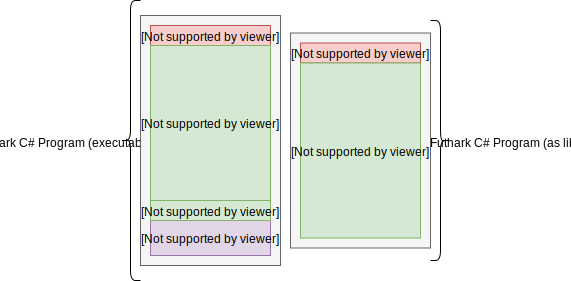
\includegraphics[scale=0.85]{chapters/figs/csharp/futharkcs_wide.pdf}
  \caption{The two possible types Futhark \csharp{} programs}
  \label{fig:futharkcsclasses}
\end{figure}

To be able to use Futhark with \fsharp{} programs, it was necessary to compile
Futhark programs to a language that \fsharp{} could work with.
Although the difference between running a compiled Futhark C- and \csharp{}
executable from the command line is negliable, a Futhark \csharp{} backend would
allow .NET projects to use Futhark libraries natively, instead of running their
Futhark calculations through seperate C or Python modules.

Because \fsharp{} has almost frictionless interoperability with \csharp{}, and \csharp{}s
imperative constructs are very close to the intermediate code that Futhark
generates for it's code generation, it was an easy decision to implement a
\csharp{} generating backend for Futhark, to accompany the already existing C-
and Python backends.

A Futhark backend must be able to do two different programs from a given Futhark
program:

First, it must be able to generate standalone executables which can take input data from the \texttt{stdin} stream, and send
the results to the \texttt{stdout} stream. Although a Futhark C, -Python or
\csharp{} executable should have equivalent functionality, their performance may
vary, and the users may alter between the versions depending on which platforms
that are available on their systems.

Second, and more interesting, it must be able to generate single file libraries
which can then be imported and used in other C, Python or \csharp{} projects, in
the same manner as any other library.

\begin{figure}[h]
  \centering
    \begin{lstlisting}[language=Futhark]
      let main (xs : []i32) : []i32 = map (+2) xs
    \end{lstlisting}
  \caption{A very small Futhark program \texttt{map2.fut}}
  \label{fig:smallfut}
\end{figure}
In example, if we compile the Futhark program in figure \ref{fig:smallfut} as a
Python library, we will be able to use it in a Python program, as showed in figure \ref{fig:smallpython}.
Likewise, we would like to be able to do the same thing in a \csharp{} or an
\fsharp{} context.
\begin{figure}[h]
  \centering
    \begin{lstlisting}[language=python]
      import numpy as np
      from map2 import map2

      xs = np.array([1,2,3])
      map2object = map2()
      xs_res = map2object.map2(xs)
      print xs_res # prints [3,4,5]
    \end{lstlisting}
  \caption{A very small Python program}
  \label{fig:smallpython}
\end{figure}

\subsection*{The anatomy of a Futhark \csharp{} program}
In figure \ref{fig:futharkcsclasses}, we see the two different ways we can
compile a Futhark program to \csharp{}. They're largely the same, except for
that the executable Futhark program must have a \texttt{Program} class with a
\texttt{Main} method defined, so that there is an entrypoint defined for the
compiled executable. Furthermore, the Futhark class in the executable version
contains an entry function which chooses what Futhark function to run (in cases
where the Futhark program has more than one entry function defined.) 

The Program class itself (as seen in figure \ref{fig:programclass}) is not especially
interesting, and does only contain a main method which initialises the Futhark
class, and calls the entry function inside the Futhark class.
For both Futhark programs, the top consists of the various imports needed for
the program.

\begin{figure}[h]
  \centering
  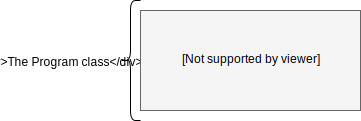
\includegraphics{chapters/figs/csharp/program_class.pdf}
  \caption{The \fshark{} compilation pipeline}
  \label{fig:programclass}
\end{figure}

This leaves us with the Futhark class itself.
Figure \ref{fig:futharkclass} shows the different parts that make up the
generated Futhark \csharp{} class. In the following sections we will walk
through the individual parts.

\begin{figure}[h]
  \centering
  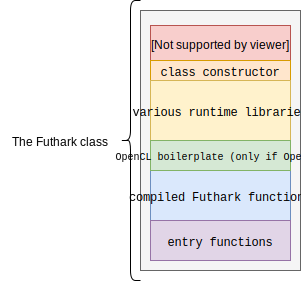
\includegraphics{chapters/figs/csharp/futhark_class.pdf}
  \caption{The layout of the \csharp{} Futhark class}
  \label{fig:futharkclass}
\end{figure}

\subsection*{Global context variables}
\label{globalcontextvariables}
Compiled Futhark programs need to keep track of several variables.
Both normal and OpenCL-enabled Futhark \csharp{} programs can take several
options when they're launched from the command line. In example,
\texttt{num\_runs} tells the Futhark runtime how many times the chosen entry
function should be executed, and the variable \texttt{runtime\_file} tells the
Futhark runtime where it should write timing information to, for example for
benchmarking purposes.

Instead of passing an argument array along throughout all the functions in the
Futhark class, like we usually would if we were writing purely functional
programs, we instead set these arguments as class variables at class
initialization, so we can refer to them everywhere throughout the rest of the class.

For non-OpenCL programs, the variables are exclusively for benchmarking and
debugging purposes. For OpenCL programs however, the global variables are vital
for the program's execution.
In an OpenCL program, the Futhark class must keep track of two extra
variables.

The struct \texttt{futhark\_context ctx} is the struct that contains the global
state of the current program's execution. Contained in the global state there is
the current list of unused but allocated OpenCL buffers on the device, kernel
handles for all the OpenCL kernels used in the Futhark program, and a counter
for the total running time of the program.
There is even another context contained in the \texttt{futhark\_context}, namely
the \texttt{opencl\_context}, which contains the current state of the device,
and also information about it's platform, it's queue and so forth.

The struct \texttt{futhark\_context\_config cfg} is similar to the
\texttt{futhark\_context}, but is only used for constructing the actual
\texttt{futhark\_context}.

\subsection*{The class constructor}
The class constructor is necessary to setup the global variables needed
throughout the Futhark class. When the Futhark program is compiled as an
executable, the command line arguments are passed to the class constructor by
the \texttt{Program} class. If the Futhark program is compiled as a library, the
programmer can pass a string array of arguments to this constructor manually.

Besides setting class variables, OpenCL-enabled versions will initialize (and
set) first the \texttt{futhark\_context\_config cfg} variable, and afterwards
the \texttt{futhark\_context} itself.

\subsection*{The various runtime libraries}
The runtime libraries are a set of seperate \csharp{} files that are written and
distributed through the Futhark compiler. When a Futhark program is compiled,
these library files are concatenated and embedded directly into the rest of the
generated code. They contain functionality which the generated Futhark programs
depend on.
The runtime libraries are the following:
\begin{description}
\item[\texttt{memory.cs}] \hfill\\
  As Futhark's stores all array values (no matter the dimensionality) as a flat one-dimensional byte arrays (with an accompanying
  array of 64-integers which denote the dimensions of the flat array), it was
  necessary to define a set of functions to interact with these byte arrays.
  I.e., \texttt{memory.cs} contains the \texttt{writeScalarArray} functions,
  which writes a scalar value to a byte array. The function is overloaded so it
  works with scalars of any integer or floating point primitive. See figure
  \ref{fig:writeScalarArray} for an example:

\begin{figure}[h]
\centering
\begin{minted}[fontsize=\small]{csharp}
void writeScalarArray(byte[] dest, int offset, double value)
{
    unsafe
    {
        fixed (byte* dest_ptr = &dest[offset])
        {
            *(double*) dest_ptr = value;
        }
    }
}
\end{minted}
\caption{\texttt{writeScalarArray} writes a value at the specified offset in
some byte array.}
\label{fig:writeScalarArray}
\end{figure}

\item[\texttt{scalar.cs}] \hfill\\
  This library contains all the scalar functions necessary for Futhark \csharp{}
  programs.
  In Futhark, arithmetic operators are defined for integers and floats of all
  sizes, and bitwise operators are defined for all integers.
  However, this is not the case in \csharp{}, where many arithmetic operators
  are only defined for 32- and 64 bit integers.
  
  If these operators are used with 8- or 16 bit operands, the operands are
  implicitly casted to 32 bit integers at compile time, which also means that
  the final result of the operation is a 32 bit integer, which doesn't has the
  right type.

  Therefore, wrapper functions must be defined for even the simplest arithmetic
  functions. I.e., integer addition in \csharp{} Futhark is actually four different
  functions:
\begin{minted}[fontsize=\small]{csharp}
static sbyte add8(sbyte x, sbyte y){ return Convert.ToSByte(x + y); }
static short add16(short x, short y){ return Convert.ToInt16(x + y); }
static int add32(int x, int y){ return x + y; }
static long add64(long x, long y){ return x + y; }
\end{minted}

  Besides, \texttt{scalar.cs} also contains the \csharp{} definitions for the various
  mathematical functions from Futhark's \texttt{math.fut}library, such as \texttt{exp},
  \texttt{sin} and \texttt{cos}.

\item[\texttt{reader.cs}] \hfill\\
  The reader contains the entire functionality for recieving function parameters
  through \texttt{stdin}. The reader reads scalars of any of the
  Futhark-supported primitives, and also arrays and multidimensional arrays of
  scalars.
  The reader also supports reading streams of binary data.
  It is only necessary for Futhark executables.
\item[\texttt{opencl.cs}] \hfill\\
  MAYBE WRITE ALL OF THIS ALSO? ALRIGHT THANKS
\end{description}

\subsection*{The compiled Futhark functions}
  The compiled Futhark functions are the Futhark Intermediate Code functions,
  expressed in the target language, and corresponds to the entry functions found
  in the entry functions-section of the Futhark class.
  Only the Futhark \texttt{entry} functions are compiled to individual functions, and
  remaining helper functions are inlined here.

  In OpenCL programs, all array functions and SOAC calls are compiled as
  individual (or fused) OpenCL kernels. Therefore, the compiled Futhark
  functions in these programs consists of mainly some scalar operations and
  memory allocations, and calls to Futhark-generated kernel wrapper functions.
  
  In non-OpenCL programs, the array functions and SOAC calls are not stored in
  seperate wrapper functions, but inlined in the Futhark functions.

\subsection*{OpenCL kernels and wrappers}
  If the Futhark program is compiled for OpenCL, all array handling function- and
  SOAC calls are compiled as OpenCL kernels. This part of the Futhark class
  has two parts:
  \begin{enumerate}
  \item The string (actually a single string in an array) \texttt{opencl\_prog}, which contains the entire
  Futhark-generated OpenCL source code for the Futhark program in question.
  This source code contains all the OpenCL kernels for the program, and is
  passed to the OpenCL device, compiled and loaded, when the Futhark class is
  initialized. Handles to the individual kernels are then stored in the \texttt{futhark\_context}.

  \item For each kernel in the \texttt{opencl\_prog}, the Futhark compiler
    generates a kernel wrapper function. These wrapper functions takes the
    kernel arguments (such as scalar values, array values and indexes) as input,
    and performs all the OpenCL specific work necessary for the actual kernel
    launch; in example setting the kernel arguments on the device, and copying
    data back and forth between host and device buffers.
  \end{enumerate}

\subsection{Entry functions}
\label{csharpentries}
Futhark's internal representation of array values are one dimensional byte
arrays (which can represent arrays of any type and dimensionality), and an
accompanying list of integers denoting the lengths of the array's dimensions.
However, Futhark does not expect it's users to pass this form of arrays as
function arguments, which is why each Futhark \texttt{entry} function has a
corresponding entry function in the final compiled code.
\\\\
To discern between Futhark functions and entry functions, the Futhark function's
name is prefixed with ``\texttt{futhark\_}'', as in for example
``\texttt{futhark\_foo}''.
Depending on whether the Futhark program is compiled as an executable or a
library, the entry function itself is then named ``\texttt{entry\_foo}'' or
just ``\texttt{foo}''.

For executables, ``\texttt{entry\_foo}'' is a function that doesn't take any
arguments. Instead, it uses the reader functions from \texttt{reader.cs} to parse the
arguments for ``\texttt{foo}'' from \texttt{stdin}, and passes them to the
Futhark function. For all array values in the arguments, the array values are
converted into Futhark representations of them.
When the Futhark function returns the result, the result is then printed to \texttt{stdout}.

For libraries, the ``\texttt{entry\_}'' prefix is dropped, and the function
just takes care of converting array arguments into and back-from their Futhark
representations.

MENTION THE INPUT ARGUMENTS SPECIFICALLY ARRAYS THAT HAVE TO BE FLATTENED FIRST

\clearpage

\section*{The \csharp{} backend, compared to the C- and Python counterparts}

%% DESCRIBE THE DIFFERENCES BETWEEN C# AND THE REST
THE PYTHON BACKEND HAS MUCH FUNCTIONALITY ENCAPSULATED IN PYOPENCL, AND DOESN'T
NEED TO DECLARE VARIABLES BEFORE SETTING THEM
LESS COMPLEX GENERATOR NEEDED AS VARIOUS OPENCL STATEMENTS ARE HANDLED
AUTOMATICALLY BY LIBRARY

C BACKEND MUST BE AWARE OF ALL SIZES AND EVERYTHING AT COMPILE TIME, WHICH MEANS
STATES MUST BE ALLOCATED THROUGH COMPLEX STRUCTS AT COMPILE TIME, AND STRUCTS
MUST BE DEFINED AT COMPILE TIME AS WELL

C ALLOWS NULL POINTERS, CS DOES NOT WHICH MEANS WE NEED PLACEHOLDER VARIABLES

CSHARP GENERATOR IS SOMEWHERE INBETWEEN AS IT IS CAN HANDLE OBJECTS WHICH CAN
CARRY STATE, FURTHERMORE DYNAMIC MEMORY ALLOCATION

% THE DIFFERENCES BETWEEN MEMORY HANDLING IN CS AND CSOPENCL
\section*{Memory management in Futhark \csharp{}}
As Futhark stores array values around in byte arrays, it is relevant to compare
the difference between how the array handling differs between Futhark's C
backend, and this \csharp{} backend.
For OpenCL programs, the memory management of \csharp{} and C is largely the
same, as the OpenCL side of these programs are the same. \csharp{} does after
all just use C bindings for it's OpenCL interactions.

However, for non-OpenCL \csharp{} programs, we have to take \csharp{}'s memory
model into consideration

C implicitly allows unsafe programming. In this case, it means interacting with system
memory by reading and writing arbitrary values from/to arbitrary locations,
designating the values and destinations as whatever type we want.
In figure \ref{fig:futharkcscene}, we see a \texttt{for}-loop that
performs a summing scan on an array of integers.
On line 6, reading from right to left, we are first creating reference to
a location in the byte array \texttt{xs\_mem\_4223}. However, as the reference
is a pointer to a byte in the array, we must recast it as an \texttt{int32\_t} pointer.
After we do this, we can finally derefer the pointer to retrieve a four byte
integer from the byte array.

We add the retrieved integer to our accumulating variable
\texttt{scanacc\_4187}, before we cast a reference in our destination byte array
as an integer pointer, and store the result there.

\begin{figure}
\centering
\begin{minted}[linenos, fontsize=\small]{c}
memblock mem_4226;
memblock_alloc(&mem_4226, bytes_4224);
int32_t scanacc_4187 = 0;

for (int32_t i_4189 = 0; i_4189 < sizze_4135; i_4189++) {
    int32_t x_4147 = *(int32_t *) &xs_mem_4223[i_4189 * 4];
    
    scanacc_4187 += x_4147;

    *(int32_t *) &mem_4226[i_4189 * 4] = scanacc_4187;
}
\end{minted}
\caption{A short snippet from a Futhark C program}
\label{fig:futharkcscene}
\end{figure}

WHY IS THIS NOT ALLOWED?

DESCRIBE TWO DIFFERENT WAYS OF DOING IT ANYHOW
1) MARSHAL
2) unsafe and fixed

what was chosen and why

% WHY THIS DESIGN

% benchmarks are available in benchmarking chapter
%% FOR CS-OPENCL, PERFORMANCE IS COMPARABLE TO C-OPENCL
%% FOR CS, PERFORMANCE IS VASTLY INFERIOR TO TO C
%%% WHY IS THAT???????????

\section*{Selection an OpenCL interface for \csharp{}}
OpenCL interaction is not a part of the .NET standard library, but several
libraries do exist for .NET/OpenCL interactions. For this thesis, I researched a
selection of these libraries, to determine which one that would fit the best for
my purposes.
As Futhark depends on being able to interface with the OpenCL platform directly,
it was necessary to find an OpenCL library for .NET which had direct bindings to
the OpenCL developer library.

The .NET libraries I took into consideration was \texttt{NOpenCL}, \texttt{OpenCL.NET} and \texttt{Cloo}.
All three libraries have been designed to aide OpenCL usage in \csharp{}
programs, by simplifying OpenCL calls behind methods GØR BEDRE.
\\
\\
\begin{description}
\item[\texttt{NOpenCL}]\hfill\\
\texttt{NOpenCL} was the first candidate for the \csharp{} backend, and had
several advantages to the other two: As per February 2018, it had been updated
within the last year, and was therefore the least deprecated library. Second,
the \texttt{NOpenCL} repository on Github contains both unit tests and
example programs.

However, \texttt{NOpenCL} is also tailored for Windows use, and therefore not a
good fit for Futhark, as Futhark is available on both Windows, Linux and Mac OS.
Furthermore, the library is not available through the NuGet
package manager, and the OpenCL API calls are needlessly complex to work with
through the library.

\item[\texttt{OpenCL.NET}]\hfill\\
\texttt{OpenCL.NET} also has a test suite, is available through NuGet, and is
used as the backend for other libraries, such as the \fsharp{} GPU library
\texttt{Brahma.FSharp}\ref{relatedwork:brahma}.

However, this library hardcoded to work on a in a Windows context, and has not been
updated for more than five years.

\item[\texttt{Cloo}]\hfill\\
\texttt{Cloo} is usable on all three
platforms, and it is available on NuGet. Furthermore, as opposed to the other two libraries, the
Cloo library contains a class with static functions that does nothing but
passing arguments on to the OpenCL library, using \csharp{}s \texttt{DllImport}
attribute. It is immediately possible to skip most of \texttt{Cloo}s features,
and just use the library for it's OpenCL bindings.

Even then, \texttt{Cloo} has not been updated within the last five years, and
probably won't be in the future either.
\\
\\
\end{description}
Given these three candidates, I chose to work with \texttt{Cloo}: It was the
only one that had the necessary OpenCL bindings readily available, and the only
one that was platform agnostic.

\subsection*{Writing a custom OpenCL bindings library}
Though \texttt{Cloo} is a good fit for Futhark \csharp{}, it is also slightly
risky to depend on a five year old unmaintained library in a modern project.
Therefore, it could be a good idea to write a smaller library similar to
\texttt{Cloo}, specifically for Futhark - or maybe even just include it with
Futhark as one of the \csharp{} runtime libraries. 

%%% Local Variables:
%%% mode: latex
%%% TeX-master: "../thesis"
%%% End:
\chapter{The \fshark{} subset}
\label{chap:fsharklanguage}
In the following chapter, we will describe the \fshark{} subset. Although the
subset is just a part of \fsharp{}, we will describe it as if it was a language
itself.

Figures \cref{fig:fsharkstatements} shows the statements available in \fshark{}, 


\begin{figure}
  \centering
  \begin{tabular}{lclr}
    $prog$ & $::=$ & $module\ prog$ & \\
           & $|$   & $prog'\ prog$  & \\
           & $|$   & $\epsilon$     & \\

    $prog'$ & $::=$ & $typealias$   & \\
            & $|$   & $fun$ & \\

    $progs'$ & $::=$ & $prog'\ progs'$   & \\
             & $|$   & $\epsilon$ & \\
    \\
    $typealias$ & $::=$ & $\texttt{type}\ v\ = t $& \\
    $module$ & $::=$ & $\texttt{module}\ v = prog'\ progs'$ & \\
    \\
    $fun$ & $::=$ & \texttt{[<FSharkEntry>]} $\texttt{let}\ id\ (v_1 : t_1)\ \ldots\ (v_n : t_n) : t = e$ & \\
        & $|$   & $\texttt{let}\ v\ (v_1 : t_1)\ \ldots\ (v_n : t_n) : t' = e,$ & \\
        &       & \hspace{1em} \textit{(for any $i \in {1..n}$, $t_i$ is not a tuple)} \\
    \\

  \end{tabular}
  \caption{\fshark{} statements}
  \label{fig:fsharkstatements}
\end{figure}



\begin{figure}
  \centering
  \begin{tabular}{lclr}
    $e$ & $::=$ & $(e)$ & Expression in parens \\
        & $|$   & $k$ & Constant \\
        & $|$   & $v$ & Variable \\
        & $|$   & $(e_0,~\ldots,~e_n)$ & (Tuple expression) \\
        & $|$   & $\{\texttt{id}_0=e_0 ; \ldots ; \texttt{id}_n=e_n\}$ & (Record expression) \\
        & $|$   & $[\vert e_0 ; \ldots ; e_n\vert]$ & (Array expression) \\
        & $|$   & $v.[e_0] \ldots .[e_n]$ & (Array indexing) \\
        & $|$   & $v.id$ & (Record indexing) \\
        & $|$   & $v.id$ & (Module indexing) \\
        & $|$   & $e_1 \odot e_2$ & (Binary operator) \\
        & $|$   & $-e$ & (Prefix minus) \\
        & $|$   & \texttt{not} $e$ & (Logical negation) \\
        & $|$   & \texttt{if} $e_1$ \texttt{then} $e_2$ \texttt{else} $e_3$ & (Branching) \\
        & $|$   & \texttt{let} $p = e_1$ \texttt{in} $e_2$ & (Pattern binding) \\
        & $|$   & $\mathtt{fun}~p_0~\ldots~p_n~\mathtt{->}~e$ & (Anonymous function) \\
        & $|$   & $e_0~e_1$ & (Application) \\

    \\
  \end{tabular}
  \caption{\fshark{} expressions}
\label{fig:fsharkexpressions}
\end{figure}

\begin{figure}
  \centering
  \begin{tabular}{@{}lclr}
    $p$ & $::=$ & $id$ & (Name pattern) \\
        & $|$   & $(p_0, \ldots, p_n)$ & (Tuple pattern) \\
  \end{tabular}
  \caption{\fshark{} patterns}
\label{fig:fsharkpatters}
\end{figure}



\begin{figure}
  \centering
  \begin{tabular}{@{}lclr}
    $t$ & $::=$ & $\texttt{int8}~|~\texttt{int16} ~|~ \texttt{int} ~ |~\texttt{int64} $ & (Integers) \\
        & $|$   & $\texttt{uint8} ~ | ~\texttt{uint16} ~|~\texttt{uint} ~|~\texttt{uint64} $ & (Unsigned integers) \\
        & $|$   & $\texttt{single} ~| ~\texttt{double}$ & (Floats) \\
        & $|$   & $\texttt{bool}$ & (Booleans) \\
        & $|$   & $(t_0 * \ldots * t_n)$ & (Tuples) \\
        & $|$   & $\{id_0:t_0;~\ldots;~id_n:t_n\}$ & (Records) \\
        & $|$   & $t~\mathtt{array}$& (Arrays) \\
    \\
  \end{tabular}
  \caption{\fshark{} types}
\label{fig:fsharktypes}
\end{figure}

\begin{figure}
  \centering
  \begin{tabular}{@{}lclr}
    $k$ & $::=$ & $n\lit{y}~|~n\lit{s}~|~n~|~n\lit{L}$ & (8-, 16-, 32- and 64 bit signed integers) \\
        & $|$   & $n\lit{uy}~|~n\lit{us}~|~n~|~n\lit{UL}$ & (8-, 16-, 32- and 64 bit unsigned integers) \\
        & $|$   & $d\lit{f}~|~d $ & (Single and double precision floats) \\
        & $|$   & $true~|~false$ & (Boolean) \\
        & $|$   & $(k_0 ,~\ldots ,~k_n)$ & (Tuple) \\
        & $|$   & $\{id_0=k_0;~\ldots;~id_n=k_n\}$ & (Record) \\
        & $|$   & $[\vert k_0 ; \ldots ; k_n\vert]$ & (Array) \\
    \\
  \end{tabular}
  \caption{\fshark{} literals}
\label{fig:fsharkliterals}
\end{figure}
\clearpage

\subsection*{\fsharp{} operators available in \fshark{}}
The \fsharp{} subset chosen for \fshark{} is described in this subsection.
\begin{figure}[h]
  \centering
\begin{description}
\item[Arithmetic operators]\hfill\\
  The set of supported arithmetic operators is addition (\texttt{+}),
  binary subtraction and unary negation (\texttt{-}), multiplication
  (\texttt{*}), division (\texttt{/}) and modulus (\texttt{\%}).
  
\item[Boolean operators]\hfill\\
  \fshark{} currently supports logical AND (\texttt{\&\&}), logical OR
  (\texttt{$||$}), less- and greater-than (\texttt{<}, \texttt{>}), less- and
  greater-or-equal (\texttt{<=}, \texttt{>=}), equality (\texttt{=}),
  inequality (\texttt{<>}) and logical negation (\texttt{not}).

\item[Special operators]\hfill\\
  \fshark{} also supports some of \fsharp{}s syntactic sugar. These operators
  might not have direct Futhark counterparts, but their applications can be
  rewritten in Futhark for equivalent functionality.
  The supported operators are back- and forward pipes (\texttt{<|} and
  \texttt{|>}), and the range operator ($e_0$ \texttt{..} $e_1$), which
  generates the sequence of numbers in the interval $[e_0,e_1]$. Note that in
  \fshark{}, the range operator must be used inside an array as so
  \texttt{[|$e_0$..$e_1$|]} so we adhere to using arrays and not lists in our
  \fshark{} programs.
\end{description}
  \caption{\fshark{} operators}
  \label{fig:fsharkops}
\end{figure}
Note that all of these operators are overloaded and defined for all integer
and floating point types in \fsharp{}.



\subsection*{\fsharp{} standard library functions available in \fshark{}}
\fshark{} supports a subset of the \fsharp{} standard library. These are
functions that are imported in \fsharp{} modules by default.

\begin{figure}[h]
  \centering
\begin{description}
\item[\texttt{id}]\hfill\\
  The identity function.

\item[Common math function]\hfill\\
  The square root function (\texttt{sqrt}), the absolute value (\texttt{abs}),
  the natural exponential function (\texttt{exp}), the natural- and the decimal
  logarithm (\texttt{log} and \texttt{log10}).
  
\item[Common trigonometric functions]\hfill\\
  Sine, cosine and tangent functions (both standard and hyperbolic):
  \texttt{sin}, \texttt{cos}, \texttt{tan}), \texttt{sinh}, \texttt{cosh} and \texttt{tanh}.
  Also one- and two-argument arctangent: \texttt{atan} and \texttt{atan2}.

\item[Rounding functions]\hfill\\
  \fshark{} supports all of \fsharp{}s rounding functions:
  \texttt{floor}, \texttt{ceil}, \texttt{round} and \texttt{truncate}.
  
\item[Number convertion functions]\hfill\\
  \fshark{} supports all of \fsharp{}s number convertion functions.
  For all the following functions $t$, $t e = e', e : t_0, e' : t$, barring
  exceptions like trying to convert a too large 64-bit integer into a 32-bit
  integer.

  The convertion functions available are \texttt{int8}, \texttt{int16}, \texttt{int}, \texttt{int64}, \texttt{uint8}, \texttt{uint16},
  \texttt{uint}, \texttt{uin64}, \texttt{single}, \texttt{double}, \texttt{bool}.
  
\item[Various common number functions]\hfill\\
  \texttt{min}, \texttt{max}, \texttt{sign} and \texttt{compare}.
\end{description}
  \caption{\fshark{} operators}
  \label{fig:fsharkfuns}
\end{figure}

Currently, bitwise operators like bitwise-AND and bitwise-OR are missing, but
they should be relatively simple to add to the \fshark{} subset, by adding them
to the set of supported operators in the \fshark{} compiler.

\subsection*{On the \fsharp{} subset selected for \fshark{}}
For selecting the \fsharp{} subset to support in \fshark{}, I chose to look at
what functions that were included in \fsharp{}'s prelude. That is, the
functions that are available in an \fsharp{} program without having to
\texttt{open} their containing module first.
Fortunately, \fsharp{} opens several modules by default of which I only
needed to look in two different ones, to be able to support a reasonable amount
of \fsharp{} built-ins in \fshark{}.

The primary module used in my supported \fsharp{} subset is the module
\texttt{FSharp.Core.Operators}.
This module contained not only the standard arithmetic described in figure
\ref{fig:fsharkops}, but also most\footnote{except for some convertion
  functions, found in \texttt{FSharp.Core.ExtraTopLevelOperators}} of the functions shown in the figure \ref{fig:fsharkfuns}.
Except for \texttt{unit} type functions like \texttt{failwith}, \texttt{exit}
and \texttt{async}, most of the functions and operators
\texttt{FSharp.Core.Operators} have direct counterparts in Futhark's prelude,
with equivalent functionality: All except for four of operators and functions chosen for
\fshark{} are in fact implemented in Futhark's \texttt{math.fut} library.
It was therefore aan obvious decision to support these functions and operators in
\fshark{}.

However, for the remaining four functions, that didn't have equivalents in
Futhark's \texttt{math.fut}, their function calls are replaced with their
identities instead.
In example, whereas the \fshark{} code
\begin{minted}{ocaml}
  exp x
\end{minted}
is written in Futhark as 
\begin{lstlisting}[language=Futhark]
  exp x
\end{lstlisting}
because the exp function is also available in \texttt{math.fut}, the \fshark{}
code
\begin{minted}{ocaml}
  cosh x
\end{minted}
is rewritten as the full hyperbolic sine function instead, as so
\begin{lstlisting}[language=Futhark]
  ((exp x) + (exp (-x))) / 2.0
\end{lstlisting}
These rewritings are not pretty to look at from a programmer's perspective, but
\fshark{}s Futhark code is not meant to be read by humans anyhow.

(MAYBE INVESTIGATE WHETHER INLINING THESE HAS PERFORMANCE PENALTIES) 

% i could have also supported limited imports

\subsection*{The correctness of the \fshark{} subset.}
When transpiling code from one language to another, it is absolutely vital that
the programmer can trust, that the resulting code in the target language is
semantically equivalent to the source code.
In \fshark{}s case, it means that any program written using the \fshark{}
subset, must have the same result no matter whether it is run natively as
\fsharp{} code, or it is run as \fshark{} compiled Futhark code.

I.e., one could imagine a programming language which had defined the function
\texttt{log} not as the natural logarithm, but instead the binary logarithm. In
such a case, the translation from that language to Futhark would still go
without a hitch, and without any type errors to hint at the impending
catastrophe.
However, the native result with the Futhark result would be wildly different.

To ensure that every operator and function in the \fshark{} subset has
equivalent results, no matter whether the \fshark{} code is run as native
\fsharp{} code, or compiled into Futhark, I have written a test suite with unit
tests for each element in the \fsharp{} subset. 


(THESE ARE NOT ACTUALLY DONE YET)
(Are unit tests enough?)

all convertion functions pass through i64. this might be a mistake, as real
supports f32 to f64

thoughts on correctness of translations
testing correctness of these translations


\chapter{FSharkPrelude}
Besides defining an \fsharp{} subset suitable for Futhark translation, it was
also imperative to create a library of SOACs and array functions for \fshark{},
to make it possible to write programs with parallel higher-order array
functions.

Similarly to how the subset of math functions chosen from \fsharp{} to include in
the \fshark{} was chosen, the SOACs and array function included in the
\texttt{FSharkPrelude} has been picked directly from the Futhark libraries
\texttt{futlib/array.fut} and \texttt{futlib/soacs.fut}. The \texttt{FSharkPrelude} doesn't
discriminate between array functions and SOACs, as maintaining and importing two
different prelude files in \fshark{} was needlessly complicated.

The \texttt{FSharkPrelude} consists of functions which are directly named after
their Futhark counterparts, and have equivalent functionality.
This prelude, together with the \fshark{} subset, is what makes up the \fshark{} language.
When \fshark{} developers are writing modules in \fshark{}, they are guaranteed
that their \fshark{} programs has the same results, no matter whether their
programs are executed like native \fsharp{} code, or compiled and executed as
Futhark.

The \texttt{FSharkPrelude} versions of Futhark functions are defined in three
different ways.
\begin{enumerate}
  \item Functions like the SOAC \texttt{map} and the array function
    \texttt{length} have direct \fsharp{} equivalents, and are therefore
    implemented as calls to \texttt{Array.map} and \texttt{Array.length}
    respectively.
    For \texttt{map} for example, we have the following definition:
    \begin{minted}{fsharp}
let Map f aa = Array.map f aa
    \end{minted}

  \item Some Futhark SOACs, like \texttt{reduce}, takes a neutral element as one of the
    arguments in their function calls, whilst their \fsharp{} counterparts
    (\texttt{Array.reduce}) does only take an operator and an array as
    arguments.
    To define the \fshark{} SOAC so that it is equivalent to the Futhark
    version, it has been defined as so:
\begin{minted}{fsharp}
let Reduce (op: 'a -> 'a -> 'a) (neutral : 'a) (xs : 'a array) =
  let xs' = Array.append [|neutral|] xs
  in Array.reduce op xs'
\end{minted}

    Other functions, like the \texttt{map} functions which takes multiple arrays as
    arguments, require a bit of assembly first. For those \texttt{map} functions,
    we zip the arguments before using \texttt{Array.map} as usual:
\begin{minted}{fsharp}
let Map5 f aa bb cc dd ee =
  let curry f (a,b,c,d,e) = f a b c d e
  let xs = Zip5 aa bb cc dd ee
  in Array.map (curry f) xs
\end{minted}

    \item Lastly, some functions does not have \fsharp{} counterparts. In
      example, we implement \texttt{scatter} using a for-loop:
\begin{minted}{fsharp}
let Scatter (dest : 'a array) (is : int array) (vs : 'a array) : 'a array =
  for (i,v) in Zip is vs do
    dest.[i] <- v
  dest
      \end{minted}
\end{enumerate}
The complete list of available SOACs and array functions is available in
appendix \ref{appendix:soacs}.

Note that calls to \texttt{FSharkPrelude} functions are caught and exchanged for
Futhark functions during the \fshark{} compilation, as described in sec \ref{kig
  kig}.

% descriptions


% WHY ALL OF THIS
\subsection*{Why is FSharkPrelude part of the \fshark{} language?}
Several of Futhark's SOACs, such as \texttt{map}, already has \fsharp{}
versions that are directly equivalent.

But there are several issues with just letting the \fshark{} programmer use 
But many of these \fsharp{} functions are
contained in 
HER KOMMER DER MERE

 1) it would be awkward to maintain a whitelist of accepted library functions,
 instead of simply handing the developer a gated library.
 1½) uncomfortable to be told function is not supported at runtime 

 2) some Array functions have subtle differences compared to their
 futhark counterparts. In example, reduce doesn't take a neutral element which
 Futhark's reduce does.

 3)


 note; FSharkPrelude cannot detect bad operators in reduce. non-commutative ops
 in reduce goes bad when parallel, så deeeeeet


 some implementations, like ZipN, are probably criminally ineffective.

 \subsection*{How \fshark{} SOACs differ from Futhark's ditto}
On a surface level, \fshark{} and Futhark SOACs are the same. After all, they
have equivalent functionality.
However, Futhark's SOACs gets special treatment in the Futhark compiler, and are
fused together where applicable.
Take for instance the short code example in figure \ref{fig:futharkfusion}.

\begin{figure}[h]
  \centering
\begin{lstlisting}[language=Futhark]
entry main : []f32 =
  let xs = iota 100
  let ys = map (f32.i32) xs
  let zs = map (+ 4.5f32) ys
  in zs
\end{lstlisting}
  \caption{A short Futhark program consisting of just SOACs}
  \label{fig:futharkfusion}
\end{figure}

For non-OpenCL programs, Futhark's compiler fuses all three expressions into one for-loop, as described
in simplified Futhark \csharp{} code in figure \ref{fig:pseudofusion}.
Similarly, in an OpenCL program, the short code example is translated into a
single kernel, as shown in figure \ref{fig:pseudokernel}.

\begin{figure}[h]
  \centering
\begin{minted}{csharp}
float[] mem = new float[100];
for (int i = 0 ; i < 100 ;i++)
{
  float res = int_to_float(i);
  res = res + 4.5f;
  mem[i] = res;
}
\end{minted}[h]
  \caption{Figure \ref{fig:futharkfusion} compiled as (simplified) non-OpenCL
    \csharp{} code.}
  \label{fig:pseudofusion}
\end{figure}

\begin{figure}
  \centering
\begin{minted}{cpp}
__kernel void map_kernel(__global unsigned byte *mem)
{
   int global_thread_id = get_global_id();
   bool thread_active = global_thread_id < 100;

   float res;

   if (thread_active) {
       res = int_to_float(global_thread_id);
       res = res + 4.5f;
   }
   if (thread_active) {
       *(__global float *) &mem[global_thread_id * 4] = res;
   }
};
\end{minted}
  \caption{Figure \ref{fig:futharkfusion}, but compiled as a simplified OpenCL kernel.}
  \label{fig:pseudokernel}
\end{figure}


In both of the compiled examples, we must first allocate a target array for our
result, but note that although we obtain three different arrays in the original
Futhark code, both of the compiled versions transform the \texttt{iota}
expression into a for-loop instead, and inserts the operators from the two
subsequent \texttt{map}s into the loop.

This is a concrete implementation Futhark fusion rules as defined in \cite{pldi17}; which states
that $(map~f) \circ (map~g) \equiv map (f \circ g)$

However, executing \fshark{} code as native \fsharp{} code will execute the
expressions as written, which means that we are allocating and writing to an
array three times, once for each line in the program.

\subsubsection*{Futhark and nested maps}
Futhark's compiler also specializes in parallelizing nested SOAC
calls\cite{pldi17}, which in example transforms nested \texttt{map} expressions into one
single \texttt{map} expression. For Futhark programs like the one in figure
\ref{fig:fsharpnested}, the resulting OpenCL program contains a single map
kernel with $i * j$ active threads.

\begin{figure}[h]
  \centering
\begin{minted}{fsharp}
let xss = map (\row ->
              map (fun col ->
                row * col
              ) <| iota j
          ) <| iota i
\end{minted}
  \caption{A nested \fshark{} program}
  \label{fig:fsharpnested}
\end{figure}

The \fsharp{} compiler doesn't make any such transformations for \fshark{} programs.

\subsection*{Arguing for Futhark-equivalent functionality}
using a test suite with both positive and negative testing

\section{Arrays in \fsharp{} versus in Futhark}
As Futhark is an array language, designing the array handling for \fshark{} was
a non-inconsequential part of the design process.
Whereas multidimensional arrays in Futhark are written as i.e. \texttt{[][]i32}
for a two dimensional integer array, their actual representation in the compiled
code is a flat array of bytes, and an array of integers denoting the lengths of
the dimensions.
Accessing the array at runtime can be done in $O(1)$, whether it's
either at some constant or a variable index (i.e. \texttt{let second\_x = xs[2]} or \texttt{let n = xs[i,j]}).
The indexes are resolved during the Futhark compilation, either as scalars, or
as a variable calculated from other variables.

RESEARCH WHETHER ``RANDOM READS'' ARE COALESCED IN A NICE WAY IN FUTHARK.

Functional languages like Haskell and \fsharp{} mainly works with lists.
In \fsharp{}, lists are implemented as singly linked lists. Nodes in the
list are dynamically allocated on the heap, and lookups take $O(n)$ time.
We cannot make multidimensional lists, but we can make lists of lists: If we
were to emulate a two dimensional list of integers in \fsharp{}, we could use
the type \texttt{int list list}. At runtime, the type would then be realized as
a singly linked list of references to singly linked list of integers.
For an \texttt{int list list} of $i \times j$ integers, we therefore have
lookups in $O(i+j)$ time.

\fsharp{} does also have arrays. The \texttt{System.Array} class itself is reference
type. If we initialize an integer array in FSharp like so: \texttt{let arr =
Array.create 10 0}, the type of \texttt{arr} is a reference to where it's corresponding
array is located in memory. As the integers contained in the array are value
types, the layout of the array referenced by \texttt{arr} is some initial array
metadata, and then the ten integers stored in sequence.

We can access the array elements on $O(1)$ time, as indexing into the array is
just done by accessing the array reference plus an index offset.
If we want to emulate multidimensional arrays with these elements, we can create
arrays of arrays (in .NET terms, these are called ``jagged arrays''). In figure
\ref{fig:jaggedarrayfsharp} we initialize a jagged array of integers.

\begin{figure}[h]
  \centering
\begin{minted}{fsharp}
let i = 8
let j = 5
let xss = Array.init i <| (Array.create j) 
  
(* xss = [|
           [|0;0;0;0;0|];
           [|1;1;1;1;1|];
           [|2;2;2;2;2|];
           [|3;3;3;3;3|];
           [|4;4;4;4;4|];
           [|5;5;5;5;5|];
           [|6;6;6;6;6|];
           [|7;7;7;7;7|];
         |]
*) 

let some_two = xss.[2].[3]

\end{minted}
  \caption{Initializing a jagged array of integers in FSharp}
  \label{fig:jaggedarrayfsharp}
\end{figure}

\texttt{xss} is an array of arrays, so \texttt{xss} is a reference to an array
in memory, which itself contains references to other arrays.
To retrieve the variable \texttt{some\_two}, we first follow the reference to
the array \texttt{xss} in memory. There we get the second element, which is a
reference to another array in memory. In this array, we read the third element,
which in this case is the 2 that we wanted.

The lookup takes $O(d)$ time\footnote{where $d$ is the number of references we
  we are chasing to get our element.}, as we access arrays in $O(1)$ time, and have to follow $d$
references to get to our element. If we just wanted a reference to the second
array in \texttt{xss}, we would be chasing the first reference to \texttt{arr},
and then return one of the references stored within.

FSharp also offers actual multidimensional arrays.
Instead of  by initiabb DO MORE HERE


comparison between arrays: multidims are represented as single objects in
memory, less cache misses. 
and so forth

\\

WE HAVE NO WAY OF KNOWING WHERE THINGS ARE ALLOCATED

SHOULD WE LOOK AT PERFORMANCE OR LANGUAGE DESIGN FIRST?


\section{Converting jagged arrays to Futhark's flat arrays,  and back again}
As mentioned in section \ref{csharpentries}, we cannot just pass jagged arrays
as arguments to the Futhark \csharp{} entry functions.
Instead, we must convert our jagged array into a flat array and an array of
integers, and pass these two objects as arguments instead.

\subsection{Analysis of FlattenArray}
The simple algorithm for this flattening is described in pseudocode in figure
\ref{fig:flattenarray}. The implemented algorithm is slightly more complex, as
it has perform various type castings, and also checks for invalid arrays such as
irregular arrays.
The implemented algorithm is available in the appendices.

When FlattenArray first is called with a jagged array as input, we don't know
how many dimensions this array has. Therefore, we recursively call FlattenArray
on the subarrays of the arrays, until these recursive calls reach a base case.
The base case is the array that does not contain array references, but primitive
values.

\begin{description}
\item[\texttt{L2}]: For a one dimensional jagged array, this branch is taken once.
  For a jagged array of $d$ dimensions, it's taken
  $\mathlarger{\prod_{n=1}^{d-1}(\text{subarrays at }d_n)}$ times.

\item[\texttt{L3}] is the base case, which takes $O(1)$ time. This is because we
are just returning a tuple with the original array, and singleton array that holds the length of the
array (creating the singleton array is also $O(1).$)

\item[\texttt{L4}]:
  For a jagged array of $d$ dimensions, this branch is taken
  $\mathlarger{\prod_{n=1}^{d-1}(\text{subarrays at }d_n)}$ times.

\item[\texttt{L5}] is the start of the recursive case. This line is called
  $O(d)$ times, $d$ being the number of dimensions in the jagged array.
  The result of \texttt{map FlattenArray array} is an array of \texttt{a} array references
  and integer array references.

\item[\texttt{L6}] MORE HERE
\item[\texttt{L7}] simply retrieves a reference to the first array in the array
  of subarray lengths. This is $O(1)$.
\item[\texttt{L8}] is by far the most costly line in the function.
  \fsharp{}s \texttt{Array.concat} function takes a sequence of arrays,
  allocates a new array, and copies each element of the old arrays into the new array.
  Each of the $n$ elements in the jagged array is copied to a new array a maximum of $d$
  times, which means we are performing $O(n*d)$ reads and writes.
  
\item[\texttt{L9}] retrieves the length of an array, and is $O(1)$.

\item[\texttt{L10}] appends a singleton array to the accumulated array of
  subarray dimensions, by first creating a singleton array, and then copy both
  the single element and the contents of the accumulated array to a third array
  of their collected length.
\end{description}

All in all, the upper bound on the \texttt{FlattenArray} algorithm is $O(n*d)$.
This is a far cry from the performance of flattening in Futhark. Flattening is
done in $O(1)$, as flattening merely calculates the product of the dimensions of
the array, and returns the result as the new single dimension of the array.


\begin{figure}[h]
  \centering
\begin{minted}[linenos]{text}
FlattenArray (array : Array of a) : (Array of b * Array of int) =
  if a is not (Array of a):
    return (array, [len(array)])
  else:
    subarrays_and_lengths = map FlattenArray array
    (subarrays, subarrays_lengths) = unzip subarrays_and_lengths
    subarray_lengths = head(subarrays_lengths)
    concatenated_subarrays = concat subarrays
    this_length = len(array)
    lengths = [this_length] @ subarray_lengths
    return (contatenated_arrays, lengths)
\end{minted}
  \caption{Flattening jagged arrays, pseudocode}
  \label{fig:flattenarray}
\end{figure}

\subsection{Analysis of UnflattenArray}
The algorithm \texttt{UnflattenArray} in figure \ref{fig:unflattenarray}
restores the flat array from the Futhark \csharp{} program, to a jagged array in \fsharp{}.
Like in \texttt{FlattenArray}, the most expensive line in the function is the
array-manipulating one. In \texttt{UnflattenArray}, it is line 7: For each
dimension in the lengths array, we chunk our data array into multiple smaller
arrays. Each of the $n$ elements in the initial array is moved to a new and smaller array
$d$ times, which makes the complexity of this algorithm $O(n*d)$.

\subsubsection*{Why UnflattenArray hinders a specific tuple type}
When an \fshark{} function is invoked, it's arguments are prepared by an
argument converter first. For scalar arguments, the argument is simply returned.
But for array arguments, we must flatten the jagged array into a tuple that
follows Futhark's array representation.

When the Futhark function returns, we then have to unflatten the Futhark arrays
back into jagged arrays. To do this, we naively look at all the values
returned by the Futhark function, and whenever we encounter a tuple of type
\texttt{('a [] * int64 [])}, we assume that this is a flat array that needs to
be unflattened.
This procedure works fine, but has one side effect: \fshark{} doesn't support
entry functions that has (\texttt{('a [] * int64 [])}) tuples in their return
types, because this type is reserved.

To circumvent this, the user is instead encouraged to return the tuple as two
separate values.

\begin{figure}[h]
  \centering
\begin{minted}[linenos]{text}
UnflattenArray (lengths : Array of int) (data : Array of a) =
  if len(lengths) = 1:
    return data
  else:
    length = head(lengths)
    lengths' = tail(lengths)
    data' = chunk_array length data 
    data'' = map (UnflattenArray lengths') data'
    return data''
\end{minted}
  \caption{Recreating a jagged array from flat array with dimensions}
  \label{fig:unflattenarray}
\end{figure}

\subsection*{An alternative solution (FSharkArrays)}
How they work

How they would alleviate the problem

Why they weren't chosen anyhow (hint; needing to pepper FSharkArray all over
code, would stand in way of idiomatic FSharp style)

\subsection*{Conclusion on arrays}
Ultimately, choosing between jagged arrays, multidimensional arrays and
FSharkArrays became a question of simplicity vs. performance.
For \fshark{}, I had the liberty to focus solely on simplicity, as \fshark{}
code is neither intended or even efficient when executed as native FSharp code.
Therefore I could choose to let \fshark{} use jagged arrays, instead of any of
the other options.

The syntax for declaring a jagged array type closely
resembles Futhark's multidimensional array syntax (take for instance FSharp's
\texttt{int [] []} versus Futhark's \texttt{[][]i32} for declaring
two-dimensional integer arrays).
The close similarities between Futhark and \fshark{} code means that \fshark{}
generated Futhark code is easier to read for debugging purposes, and likewise
makes Futhark code easier to port to \fshark{}.

%%% Local Variables:
%%% mode: latex
%%% TeX-master: "../thesis"
%%% End:
\chapter{The \fshark{} Wrapper}
In this chapter we will first demonstrate how to compile and use an \fshark{}
module within an \fsharp{} project.
We will then delve further into how and why compiled \fshark{} functions are actually
invoked through through a wrapper class called the \fsharkwrapper{}.

Finally, we will discuss the performance disadvantages that comes with the
current implementation of the \fshark{} wrapper.

\section{Using the \fshark{} Wrapper}
\label{sec:fsharkcompiler}
Although \fshark{} code can be executed directly in \fsharp{} as normal
\fsharp{} code, our benchmarks in section~\ref{sec:fsharkgpubenchmarks} shows
that compiling our \fshark{} code to Futhark GPU modules gives us performance
increases by several orders of magnitudes (from $\times 100~\text{to}~\times 1000$).

We therefore need to implement a wrapper which enables us to compile our
\fshark{} programs as well as utilize them in our \fsharp{} programs.
\subsection{Another short \fshark{} module}
Below we see a simple \fshark{} module that we
want to compile into a GPU kernel and use in our \fsharp{} program.

\begin{minted}[linenos]{fsharp}
module ExampleModule
open FSharkPrelude

let saxpy (a : int) (x : int) (y : int) : int =
  a*x+y

let getArrayPair (a : int) : (int array * int array) =
  let xs = Iota a
  let n = Length xs
  let ys = Rotate (n / 2) xs
  in (xs, ys)

[<FSharkEntry>]
let entry (a : int) : int array =
  let (xs, ys) = getArrayPair a
  let res = Map2 (saxpy a) xs ys
  in res
\end{minted}

Line by line, this module does the following:\\
\textbf{L1:} We define the name of this module as \texttt{ExampleModule}. If we
want to use this module in an \fsharp{} program without compiling it as
\fshark{} first, we can refer to this module by this name.
\\
\textbf{L2:} We open \fshark{}s standard library \texttt{FSharkPrelude} in this
module, so we can access the standard functions in the \fshark{} module.
In this module, we are using the standard functions \texttt{Iota}, \texttt{Length}, \texttt{Rotate} and \texttt{Map2}.
\\
\textbf{L4-5:} We define the function \texttt{saxpy}.
\\
\textbf{L7-11:} We define the function \texttt{getArrayPair}.
\\
\textbf{L8:} \texttt{Iota a} returns the integer array of the numbers from $0$
up to, but not including, $a$.
\\
\textbf{L9:} \texttt{Length xs} returns the length of the array \texttt{xs}.
\\
\textbf{L10:} \texttt{Rotate n} rotates the contents of an array n places in
either the right or left direction.\\
For example, \texttt{Rotate 2 [1;2;3;4;5;6] = [5;6;1;2;3;4]},\\
and \texttt{Rotate (-2) [1;2;3;4;5;6] = [3;4;5;6;1;2]}
\\
\textbf{L11:} Here we return the pair of arrays \texttt{(xs, ys)}.

\textbf{L13-17:} We define the entry function \texttt{entry}.\\
\textbf{L15:} We call \texttt{getArrayPair} to get two arrays.\\
\textbf{L16:} We use \texttt{Map2} to map the curried function \texttt{(saxpy
  a)}
over the arrays \texttt{xs} and \texttt{ys}.

For two arrays $\mathtt{xs} =
[\mathtt{x}_1,~\mathtt{x}_2,~\ldots,~\mathtt{x}_n]$ and $\mathtt{ys} =
[\mathtt{y}_1,~\mathtt{y}_2,~\ldots,~\mathtt{y}_n]$,\\
$\mathtt{Map2}~\mathtt{(saxpy~a)}~\mathtt{xs}~\mathtt{ys} =
[\mathtt{saxpy~a}~\mathtt{x}_1~\mathtt{y}_1,
\mathtt{saxpy~a}~\mathtt{x}_2~\mathtt{y}_2,\ldots,~\mathtt{saxpy~a}~\mathtt{x}_n~\mathtt{y}_n]$.
\\
\\
\textbf{L17:} The entry function returns the result of the call to \texttt{Map2}.

This concludes the short \fshark{} module.

\subsection{Compiling and using the short \fshark{} module}
\label{compilingandusingfsharkmodule}
With our \fshark{} module ready, we now proceed to compile, load and use it.
This is shown in figure \ref{fig:fsharkusageexample}.
\begin{figure}[H]
  \centering
    \begin{minted}[linenos,breaklines]{fsharp}
module FSharkExample
open FShark.Main

[<EntryPoint>]
let main argv =
  let wrapper = 
    new FSharkWrapper(
      libName="ExampleModule",
      tmpRoot="/home/mikkel/FShark",
      preludePath= "/home/mikkel/Documents/fshark/FSharkPrelude/bin/Debug/FSharkPrelude.dll",
      openCL=true,
      unsafe=true,
      debug=false
      )
  wrapper.AddSourceFile "ExampleModule.fs"
  wrapper.CompileAndLoad
  let a = 1000000
  let result = wrapper.InvokeFunction("entry", a) :?> int array
  printfn "Mapping (+2) over %A gives us %A" xs xs'
  0
    \end{minted}
  \caption{An F\# program using \fshark{}}
  \label{fig:fsharkusageexample}
\end{figure}

Let us now explain line by line what is happening in the figure:\\
\textbf{L6:} We begin by constructing an instance of the \fshark{}Wrapper. It has the following
mandatory arguments:

\begin{description}
\item[\texttt{libName}]\hfill\\
  This is the library name for the \fshark{} program. In the final Futhark
  \texttt{.cs} and \texttt{.dll} files, the main class will have the same name
  as the \texttt{libName}. This doesn't really matter if \fshark{} is just used
  as a JIT compiler, but it's good to have a proper name if the user only wants
  to use the compiler parts of \fshark{}.

\item[\texttt{tmpRoot}]\hfill\\
  The \fshark{} compiler works in its own temporary directory. This argument must
  point to a directory where F\# can write files and execute subprocesses
  (Futhark- and C\# compilers) which also has to write files.
  
\item[\texttt{preludePath}]\hfill\\
  The \fshark{} compiler needs the FShark prelude available to compile FShark
  programs. 

\item[\texttt{openCL}]\hfill\\
  Although Futhark (and therefore \fshark{}) is most effective on OpenCL-enabled
  computers, the benchmarks in \ref{sec:fsharkgpubenchmarks} still show a significant
  speed increase for non-OpenCL Futhark over native F\# code.
  Therefore, \fshark{} is also available for non-OpenCL users. Use this flag to
  tell \fshark{} whether Futhark should compile C\# with or without OpenCL.
  
\item[\texttt{unsafe}]\hfill\\
  For some Futhark programs, the Futhark compiler itself is unable to tell
  whether certain array operations or SOAC usages are safe, and will stop the
  compilation, even though the code should (and does) indeed work.
  To enable these unsafe operations, pass a \texttt{true} flag to the compiler.

\item[\texttt{debug}]\hfill\\
  Passing the debug flag to the \fshark{} compiler enables various runtime
  debugging features, for instance benchmarking the time it takes to run various
  parts of the compiler.
\end{description}

\textbf{L15:} Now we can pass a source file to the \fshark{} wrapper. \\
\textbf{L16:} We tell the wrapper to compile the source file that we have added
to the wrapper object, and load the compiled library into the wrapper
afterwards.\\
\textbf{L17:} As our entry function defined in the program in figure
\ref{fig:fsharkusageexample} takes an integer as argument, we define an integer
variable we can pass to it.\\
\textbf{L18:} We use the wrapper to invoke the entry function from the compiled
and loaded library, using our previously declared \texttt{a} as the only
argument. As the \fshark{} wrapper uses reflection to dynamically load compiled
libraries at runtime, we are not able to statically determine what type of
result we will get from the \texttt{InvokeFunction} call. Therefore, we use F\#s
downcast operator \texttt{(:?>)} to declare the return value as an \texttt{int
  array}.

If we are in doubt of which type to downcast to, we can always lookup the return
type by reviewing the \fshark{} module's source code. We can downcast to any of
the types usable in \fsharp{}, including tuples and arrays.

\section{On the design decisions of the \fshark{} wrapper}
To summarize, the current design of \fshark{} usage is dependent on a
wrapper object, which for all \fshark{} projects must compile and load 
the input \fshark{} modules once, and, afterwards, it must pass arguments 
from \fsharp{} to the resulting GPU kernels by using .NET reflection.
This design has several costs for both usability and performance, and we will
here discuss some of these costs, and what we could do to alleviate them in the
future.

\subsection{Compiling and loading \fshark{} modules at every startup}
At this time, \fshark{} works by compiling and loading \fshark{} modules just in
time before they are needed in the containing \fsharp{} project. However, this
is more often than not redundant work. For the developer who is using \fshark{} to develop
prototypes of \fshark{} GPU kernels, it is of course beneficial to continuously
recompile the \fshark{} program under development to verify that changes are being
made.

However, when the \fshark{} program is finished and ready to be used in
projects, it isn't necessary to compile it again.

\subsubsection{How much time do we spend on compiling and loading the \fshark{} modules?}
If we, instead of loading the compiled \fshark{} GPU kernels through the
\fshark{} wrapper, just open the compiled kernel libraries as any other
\csharp{} \texttt{.dll} file, we can circumvent the \fshark{} compiler
completely, and use the compiled kernel directly.

For the two benchmarks \texttt{LocVolCalib} and \texttt{nbody}(see sec
\ref{sec:fsharkgpubenchmarks}), we have compared the time cost of the two different
approaches. In figure \ref{benchmarkcalculations} we see how the time is spent
in the two different methods.
\begin{figure}[H]
  \centering
  \begin{tabular}{@{}l c r c l c r}
 Parsing \fshark{} code using \fsharp{} parser          & &   217984 ms & $\vrule$ & & & \\
    Converting \fsharp{} declarations to FSharkIL       & &+   19129 ms & $\vrule$ & & & \\
 Converting FSharkIL to Futhark source code             & &+   98949 ms & $\vrule$ & & & \\
 Compiling Futhark to \csharp{} with \texttt{futhark-cs}& &+ 8037165 ms & $\vrule$ & & & \\
 Compiling \csharp{} code using \csharp{} compiler      & &+  999251 ms & $\vrule$ & & & \\
 Loading compiled \csharp{} class using reflection      & &+  101601 ms & $\vrule$ & & & \\
 Loading and constructing class from library & & & $\vrule$ & & &
  \end{tabular}
  \caption{Time spent on making LocVolCalib available in \fshark{}-using
    program}
  \label{benchmarkcalculations}
\end{figure}

So the dynamic compilation process takes about $10$ seconds, while running the
accelerated program on the largest dataset takes only a couple of seconds.

MORE BENCHMARKS

WE ARE OBVIOUSLY WASTING TIME

\subsubsection{Suggestions for changes}
We have two main suggestions for change.\\
1) The easiest way would be to add a \texttt{AddModulePath} function to the
\fshark{} wrapper. The benchmarks show that we aren't spending that much more
time when loading compiled assemblies into \fsharp{} using reflection, than if
we opened the assembly as a library in the project.

Therefore, we could add a function that takes a path to a compiled \fshark{}
module, and loaded the path's target into the wrapper.

2) We could also go for a second, more permanent solution. Instead of relying on
\fsharp{}s reflection functionality to load our compiled assemblies into scope
dynamically, we could redesign the \fshark{} use case itself, so that it uses
just the compiler, and not the wrapper.

In this case, the new use case would be to compile the \fshark{} modules using
the \fshark{} compiler, and then manually reference- and open them in \fsharp{} projects.
This would not only remove the repeated module compilation, but also let us use
static typing with the compiled \fshark{} modules, enabling autocompletion and
type checking for function arguments, and also removing the need to manually
downcast the \fshark{} invokation results.

\subsection{The overhead of invoking GPU kernels}
\label{invocationoverhead}
The second issue with the current approach is, that every single call to a
\fshark{} function carries significant overhead for copying data back and forth
between CPU and GPU buffers.
This is a problem when we are chaining together GPU function calls: that is when
we take the array output of function $f$ and use it as an argument for function
$g$ without any changes to it.

In figure \ref{fig:witharraycopying} we see a chain of three calls to a compiled \fshark{} module. 
Although we are calling the second function with the result from the first
function together with another array, and calling the third function with result
from the second function, we are still moving the results from the GPU buffers to our system RAM between each call, and deallocating
the buffers on the GPU, even though we are going to reallocate them soon
thereafter.

\begin{figure}[H]
  \centering
  \includegraphics[scale=1.15]{chapters/figs/witharraycopying.pdf}
  \caption{Buffers are copied back and forth between CPU and GPU between calls}
  \label{fig:witharraycopying}
\end{figure}


In the future, we could eliminate this overhead by allowing the compiled Futhark functions
to opaque arrays instead of actual data arrays. Opaque arrays are merely
references to already allocated GPU buffers, and can be resolved into actual
data arrays only when the data is needed in the remaining program. 

We could then also have multiple versions of the compiled Futhark functions; one
version that takes an actual data array as input, and one that can use a
reference to a GPU buffer instead.

In this case, we could wait until after the three function calls to actually
copy the referenced GPU buffer back to the system RAM. This would strongly reduce the
number of copies back and forth between the GPU and the system RAM:
Instead of the allocations/deallocations increasing linearly with the number of
chained GPU kernel calls, we can make do with one allocation and one
deallocation between system RAM and GPU, pr. chain, as in figure \ref{fig:withoutarraycopying}
\begin{figure}[H]
  \centering
  \includegraphics[scale=1.15]{chapters/figs/withoutarraycopying.pdf}
  \caption{Buffers aren't copied between CPU and GPU unless necessary}
  \label{fig:withoutarraycopying}
\end{figure}

This functionality is already implemented in Python's \texttt{PyOpenCL} library,
and is used in Futhark programs that are compiled as Python libraries.
\clearpage

\chapter{The \fshark{} Compiler}
\label{chap:fsharkcompiler}
In this chapter, we present the \fshark{} compiler pipeline.
We first present the compiler architecture, and followingly describe the four
parts of the compiler piece by piece, with accompanying compilation and
translation examples.

\section{The \fshark{} compiler architecture}

At this point in the report, we are able to generate GPU-accelerated
computational kernels for \csharp{}. We
have also defined a language for writing GPU kernels using \fsharp{}, and we have
offered several methods of integrating these compiled \csharp{} kernels in
\fsharp{} projects. What remains is to build a compiler, that takes \fshark{}
code as input, and returns a compiled \csharp{} library that runs GPU
computational kernels.

In practice, we need to build an architecture that supports the functionality
defined in figure \ref{fig:fsharkcompilerarchitecture}.

\begin{figure}[H]
  \centering
  \includegraphics[scale=1.15]{chapters/figs/compilerarchitecture.pdf}
  \caption{The complete architecture from \fshark{} source code to compiled
    \csharp{} program.}
  \label{fig:fsharkcompilerarchitecture}
\end{figure}


\section{The FSharp parser}
Parsing and building a regular \fsharp{} program is trivial when using official build tools like
\texttt{msbuild} or \texttt{fsharpc}.
But in the case of \fshark{}, we are not interested in the final output of the
\fsharp{} compiler. Instead, we use only part of the \fsharp{} compiler's
pipeline: By passing our \fshark{} source code through the \fsharp{} compiler's
parser features, we retrieve its corresponding Typed Abstract Syntax Tree.

The Typed Abstract Syntax Tree (TAST) contains the function and value declarations that makes up 
our \fshark{} program.
The Typed Abstract Syntax Tree is merely an AST that already has tagged all the
contained expressions with their respective types.\\
We take this TAST and pass it on into the \texttt{FSharkCompiler}.

As the F\# Software Foundation offers the official F\# Compiler as a freely
available NuGet package for F\# projects, we can use this package
\texttt{FSharp.Compiler.Services} to parse the entire input \fshark{} program and
give us a Typed Abstract Syntax Tree of the FSharp expressions therein, instead
of writing our own parser. So as the \fsharp{} parser part of the pipeline amounts to calling some library
functions from an imported library, we will not use more time on this part.

\section{The \fshark{}Compiler}
For the \fshark{}Compiler, we need to build a module that takes an \fsharp{}
TAST as input, and returns the corresponding program as written in an
intermediate language defined for \fshark{}, called \fshark{}IL.\\
The declarations in the TAST are called \texttt{FSharpDecl}s, and in \fshark{}
we work with two kinds of \texttt{FSharpDecl}s.

The first kind of FSharpDecl that \fshark{} supports is the \texttt{FSharpDecl.MemberOrFunctionOrValue}, which are
declarations of members, functions and values. We don't use members in
\fshark{}, as they are for object oriented \fsharp{} programming, but we do use
functions and values. For all intents and purposes, \fsharp{} values are just
functions without arguments.

The other kind is the \texttt{FSharpDecl.Entity}. Entities are \fsharp{}
declarations that are neither functions or values
themselves, but instead alterations to the present \fsharp{} program. 
The \fshark{}Compiler supports three different entities.

In total, this means that our intermediate language must also support four
different declarations, which are the \texttt{FSharkDecl}s. These are shown in
figure \ref{fig:fsharkdecls}.

\subsection{FSharpDecl.Entity}
The \fshark{}Compiler supports three different entities.
\begin{description}
\item[FSharpRecords] are standard record types, and can be translated to
  Futhark records with ease.
  This entity has an empty \texttt{FSharpImplementationFileDeclaration list}.
\item[FSharpAbbreviations] are type abbreviations, and are easily translated
  into Futhark type aliases.
  This entity has an empty \texttt{FSharpImplementationFileDeclaration list}.
\item[FSharpModules] are named modules which contains subdeclarations. In
  \fshark{} we don't support parameterized modules, so in reality the just work
  as namespaces for functions and values.
  The \fshark{} compiler supports building FShark modules, but current
  limitations demands that modules are flattened when compiled to Futhark.
  This also means that function name prefixes in function calls are stripped
  when compiled to Futhark.

  An example of this module flattening is shown below.

\begin{minted}{fsharp}
module Vec3 =
    type Vec3single = {x:single ; y:single ; z:single}
    let plus (a : Vec3single) (b : Vec3single) : Vec3single =
        {x=a.x+b.x; y=a.y+b.y; z=a.z+b.z}
            
type vec3 = Vec3.Vec3single
type mass = single
type position = vec3
type acceleration = vec3
type velocity = vec3
\end{minted}

\begin{lstlisting}[language=Futhark]
type Vec3single = {x : f32, y : f32, z : f32}
let plus (a : Vec3single) (b : Vec3single) : Vec3single =
  {x=((a.x + b.x)), y=((a.y + b.y)), z=((a.z + b.z))}

type vec3 = Vec3single
type mass = f32
type position = Vec3single
type acceleration = Vec3single
type velocity = Vec3single
\end{lstlisting}

  Here, the \texttt{Vec3} module is flattened
  and made part of the outer scope of the file. 
  Due to time constraints, this current solution was chosen.
  The solution does introduce the danger of namespace collisions. for example,
  we could get in trouble by having a function further down which was also called \texttt{plus}.

  A later version of the \fshark{}Compiler could very well contain a better
  solution to the module problem, either by translating \fshark{} modules to
  Futhark modules, or at least by naming the flattened module declarations in a
  special way; for example by keeping the containing module's name in the flattened
  declarations' name, like in the example below:
\end{description}

\begin{minted}{fsharp}
module Vec3 =
    type Vec3single = {x:single ; y:single ; z:single}
    let plus (a : Vec3single) (b : Vec3single) : Vec3single =
        {x=a.x+b.x; y=a.y+b.y; z=a.z+b.z}
            
type vec3 = Vec3.Vec3single
\end{minted}

\begin{lstlisting}[language=Futhark]
type Vec3_Vec3single = {x : f32, y : f32, z : f32}
let Vec3_plus (a : Vec3_Vec3single) (b : Vec3_Vec3single) : Vec3_Vec3single =
  {x=((a.x + b.x)), y=((a.y + b.y)), z=((a.z + b.z))}

type vec3 = Vec3_Vec3single
\end{lstlisting}



\subsection{\fsharp{} expressions}
\label{sec:fsharpexprs}
An \fsharp{} function or value is not without its accompanying \fsharp{}
expression. The \fsharp{} compiler compiles these \fsharp{} expressions into
\texttt{FSharpExpr}s, which we can parse ourselves, and rewrite as \fshark{}IL expressions.
In figure \ref{fig:fsharpexprs0} we see three different \fsharp{} expressions,
and their representations as \texttt{FSharpExpr}'s.

For the first example, we just create a tuple literal. In the
\texttt{FSharpExpr} version, we see how the literal is created using
\texttt{NewTuple}. \texttt{NewTuple} takes a list of \texttt{FSharpExpr}s as
arguments. In this case, we are using two constants, each of which takes some
primitive object, and the .NET type of that object.

In the second example, we use the \texttt{Let} expression. Semantically, \texttt{Let} takes a
name $n$ and two expressions $e_1$ and $e_2$, and exchanges every instance of
$n$ in $e_2$ with $e_1$.
Then we encounter two \texttt{Let}-expressions that we didn't write ourselves.
That is because the \fsharp{} compiler turns tuple assignments into chains of
\texttt{Let} expressions instead. Here, we use \texttt{TupleGet} to get each
field of the tuple.

Finally, we use a typed instance of the \texttt{Call} expression to call the
overloaded function \texttt{Plus} as the integer version of the plus function,
giving it the two variables \texttt{Value a} and \texttt{Value b} as arguments.

In the third example, we see the \texttt{Lambda} expression in use. \texttt{Lambda} takes
a list of variables (in the form of name/type pairs), and an \texttt{FSharpExpr}. In this case,
\texttt{Lambda} only has one variable.\\
The innermost expression here is the \texttt{Application} expression.
\texttt{Application} takes a function or a lambda, and a list of arguments, and
applies the list of arguments one by one to the function or lambda.

\begin{figure}[H]
  \centering
\begin{minted}{fsharp}
  // example 1
  (79, 42.0f)

  // example 2
  let tuple = (79, 42.0f)
  let (a,b) = tuple
  in a + a

  // example 3
  let a = 2.0f
  let foo = fun x -> x + 3.0f
  in foo a
\end{minted}

\begin{minted}{lisp}
  ; example 1
  NewTuple ([Const(79, System.Int32), Const(42.0f, System.Single)])

  ; example 2
  Let tuple (NewTuple ([Const(79, System.Int32), Const(42.0f, System.Single)]))
  ( 
    Let a (TupleGet 1 tuple) 
    (
      Let b (TupleGet 2 tuple) 
      (
        Call Plus System.Int32 
          ([Value a, Value b])
      )       
    )
  )

  ; example 3
  Let a Const(2.0f, System.Single)
  (
    Let foo (Lambda ([(x, System.Single)]) 
                   (Call Plus System.Single 
                     ([Value x, Const(3.0f, System.Single)])
                   ))
    (
      Application foo ([Value a])
    )

  )
\end{minted}
  \caption{Three \fsharp{} expressions, and their representation as
    \texttt{FSharpExpr}s}
  \label{fig:fsharpexprs0}
\end{figure}

The entire set of \texttt{FSharpExpr}s used in the \fsharkcompiler{} is
available in figure \ref{fig:fsharpexprs1}, and the entire set of .NET types used in the \fshark{}Compiler is
available in figure \ref{fig:fsharptypes0}.

\subsection{Translating from FSharpExprs to \fshark{}IL}
Now that we have the \fsharp{} expressions and types in order, we can translate
them into our \fshark{} intermediate language, \fshark{}IL.

Continuing the example from figure \ref{fig:fsharpexprs0}, we will see three
examples of such translations in figure \ref{fig:fsharpexprs2}.
The expressions as written in \fshark{}IL happens to look very much like \fshark{}s own
expressions, except for one thing. In \fsharp{}, infix operators are translated
into normal function calls at compilation.

Therefore, the \fshark{}Compiler detects these specific function calls (the calls to infix operators), and 
translates them back into infix operations.
Although it would possible to treat infix operators as functions in the
\fshark{} generated Futhark code, we have chosen to write the
operator calls as infix operations, for readability.

\begin{figure}[H]
  \centering
\begin{minted}{lisp}
  ; example 1
  NewTuple ([Const(79, System.Int32), Const(42.0f, System.Single)])

  ; example 2
  Let tuple (NewTuple ([Const(79, System.Int32), Const(42.0f, System.Single)]))
  ( 
    Let a (TupleGet 1 tuple) 
    (
      Let b (TupleGet 2 tuple) 
      (
        Call Plus System.Int32 
          ([Value a, Value b])
      )       
    )
  )

  ; example 3
  Let a Const(2.0f, System.Single)
  (
    Let foo (Lambda ([(x, System.Single)]) 
                   (Call Plus System.Single 
                     ([Value x, Const(3.0f, System.Single)])
                   ))
    (
      Application foo ([Value a])
    )

  )
\end{minted}
\begin{minted}{lisp}
  ; example 1
  Tuple ([Const(79, FInt32), Const(42.0f, FSingle)])

  ; example 2
  LetIn tuple (Tuple([Const(79, FInt32), Const(42.0f, FSingle)]))
  ( 
    LetIn a (TupleGet tuple 1) 
    (
      LetIn b (TupleGet tuple 2) 
      (
        InfixOp Plus FInt32 (Var a) (Var b)
      )       
    )
  )

  ; example 3
  LetIn a Const(2.0f, FSingle)
  (
    LetIn foo (Lambda ([(x, FSingle)]) 
                   (InfixOp Plus FSingle (Var x) (Const(3.0f, FSingle)))
              )
    (
      Application foo ([Var a])
    )

  )
\end{minted}
  \caption{Three \texttt{FSharpExpr}s expressions, and their representation as \texttt{FSharkExpr}s}
  \label{fig:fsharpexprs2}
\end{figure}

The complete set of rules for translating .NET types to \fshark{} types are
available in figure \ref{fig:.nettofsharktypes}, and the complete set of rules
for translating \texttt{FSharpExpr}s to \texttt{FSharkExpr}s are shown in figure \ref{fig:fsharpexprstofsharkexprs}.

With the \texttt{FSharpExpr}s translated to \texttt{FSharkExpr}s, we can pass
the entire program as written in \fshark{} intermediate code onto the next part
of the compiler pipeline; the \fshark{}Writer.
\section{The \fshark{}Writer}
The \fshark{}Writer takes programs written in \fshark{}s intermediate language,
and translates them into valid Futhark source code.

Continuing the example from figure \ref{fig:fsharpexprs2}, we will see three
examples of such translations in figure \ref{fig:fsharkexprs3}.

The complete set of \fsharkexpr{}-to-Futhark rules are shown in figure
\ref{fig:fsharkexprstofutharkcode}, and the rules for translating \fsharkil{}-types to
Futhark-types are shown in figure \ref{fig:fsharkiltofutharktypes}.

\begin{figure}[H]
  \centering
\begin{minted}{lisp}
  ; example 1
  Tuple ([Const(79, FInt32), Const(42.0f, FSingle)])

  ; example 2
  LetIn tuple (Tuple([Const(79, FInt32), Const(42.0f, FSingle)]))
  ( 
    LetIn a (TupleGet tuple 1) 
    (
      LetIn b (TupleGet tuple 2) 
      (
        InfixOp Plus FInt32 (Var a) (Var b)
      )       
    )
  )

  ; example 3
  LetIn a Const(2.0f, FSingle)
  (
    LetIn foo (Lambda ([(x, FSingle)]) 
                   (InfixOp Plus FSingle (Var x) (Const(3.0f, FSingle)))
              )
    (
      Application foo ([Var a])
    )

  )
\end{minted}
\begin{lstlisting}[language=Futhark]
-- example 1
(79i32, 42.0f32)

-- example 2
let tuple = (79i32, 42.0f32) in
let a = tuple.1 in
let b = tuple.2 in
a i32.+ b

-- example 3
let a = 2.0f32 in
let foo = (\(x : f32) -> x i32.+ 3.0f32) in
in foo a
\end{lstlisting}
  \caption{Three \texttt{FSharkExpr}s expressions translated to Futhark by
    \fshark{}Writer}
  \label{fig:fsharkexprs3}
\end{figure}

The \fshark{}Compiler creates a temporary folder at the temporary root folder\footnote{see the \texttt{tmpRoot} variable in sec \ref{compilingandusingfsharkmodule}}
that was passed as an argument when initializing the \fshark{}Wrapper, and
writes the finished string of Futhark source code to a Futhark file in this
directory.
The name of the Futhark file is taken from the \texttt{libName} variable we
passed to the \fshark{}Wrapper at its initialization.

\subsection{The Futhark-to-\csharp{} compiler}
The \fshark{}Wrapper now calls the Futhark-to-\csharp{} compiler
\texttt{futhark-cs}. If we named our \fshark{} module ``MyLib'', the command
used be like shown below:\\
\begin{lstlisting}[language=sh]
$ futhark-cs --library -o MyLib.dll MyLib.fut
\end{lstlisting}

\texttt{futhark-cs} compiles a \csharp{} dynamically linked library and writes
it to \texttt{MyLib.dll}, and also writes the \csharp{} source code from the
Futhark compilation to \texttt{MyLib.cs}.

This marks the end of the \fshark{} compilation process.


\section{Design choices in writing the FShark Compiler}
To implement the \fsharkcompiler{}, we had the choice between implementing a
lexer and parser manually, or using \fsharp{}'s own compiler as a parser library.
Furthermore, \fsharp{}'s Typed Abstract Syntax Trees shows the types of any
functions and operators used in an \fsharp{} program. This means, that even for
the program shown in \ref{fig:shortprogrammmm}, the \fsharp{} compiler's type
inference tells us that the plus operator used in the expression on line 3 is
the \texttt{int} plus operator.

\begin{figure}[H]
  \centering
\begin{minted}{fsharp}
let x = 7
let y = 9
in x + y
\end{minted}
  \caption{A short \fsharp{} program that uses type inference to decide the
    types of the plus-operator's operands.}
  \label{fig:shortprogrammmm}
\end{figure}
If we were to implement our own \fsharp{} parser, we would not only have to
implement the lexer and parser ourselves, but also type inference.

I chose to use \fsharp{}'s own compiler as it gave me all this functionality for
free, out of the box.

\clearpage
\section{Figures}
\begin{figure}
  \centering
\begin{tabular}{@{}l c l}% to \linewidth {l c X}
  $Decl$ & $:=$    & $\lit{FSharkRecord}([(field_1, decl_1),\ldots,(field_n, decl_n)])$ \\
         & $\vert$ & $\lit{FSharkTypeAlias}(name, \tau)$ \\
         & $\vert$ & $\lit{FSharkModule}(name, [decl_1,\ldots, decl_n])$\\
         & $\vert$ & $\lit{FSharkVal}(name, [\tau_1, \ldots, \tau_n], [arg_1, \ldots, arg_n], \tau_{return}, e)$\\
  ~ \\
\end{tabular}
\caption{The four possible \texttt{FSharkDecl}s.}
\label{fig:fsharkdecls}
\end{figure}

\begin{figure}
  \centering
\begin{tabular}{l c l}% to \linewidth {l c X}
   $\tau$& $=$     &  \texttt{System.Int8} \\
         & $\vert$ &  \texttt{System.Int16} \\
         & $\vert$ &  \texttt{System.Int32} \\
         & $\vert$ &  \texttt{System.Int64} \\
         & $\vert$ &  \texttt{System.UInt8} \\
         & $\vert$ &  \texttt{System.UInt16} \\
         & $\vert$ &  \texttt{System.UInt32} \\
         & $\vert$ &  \texttt{System.UInt64} \\
         & $\vert$ &  \texttt{System.Single} \\
         & $\vert$ &  \texttt{System.Double} \\
         & $\vert$ &  \texttt{System.Boolean} \\
         & $\vert$ &  \texttt{System.Array} $\tau$ \\
         & $\vert$ &  \texttt{System.Tuple} $(\tau_1 \times \ldots \times \tau_n)$ \\
\end{tabular}
\caption{The .NET types used in the \fshark{}Compiler}
\label{fig:fsharptypes0}
\end{figure}


\begin{figure}
  \centering
  \begin{tabular}{@{}l c l}% to \linewidth {l c X}
e & $=$ &   Const(obj, $\tau$) \\
 & $\vert$ &   Value(v) \\
 & $\vert$ &   AddressOf(v) \\
 & $\vert$ &   NewTuple($\_, [e_0,...,e_n]$) \\
 & $\vert$ &   NewRecord([$(v_0 , e_0),~\ldots,~(v_n , e_n)$]) \\
 & $\vert$ &   NewArray($\tau, [e_0,...,e_n]$) \\
 & $\vert$ &   TupleGet($\_$, i, e) \\
 & $\vert$ &   FSharpFieldGet($e, \_, field$) \\
 & $\vert$ &     Call($\_, \lit{GetArray}, \_, nil, [e_0, e_1]$) \\
 & $\vert$ &     Call($\_, name, \_, nil, [e_0, \ldots, e_n]$) \\
 & $\vert$ &     Call($\_, name, \_, \tau, [e_0, \ldots, e_n]$) \\
 & $\vert$ &     Call($\_, infixOp, \_, \tau, [e_0, e_1]$) \\
 & $\vert$ &     Call($\_, unaryOp, \_, \tau, [e_0]$) \\
 & $\vert$ &   Let($p, e_0, e_1$) \\
 & $\vert$ &   IfThenElse($e_0, e_1, e_2$) \\
 & $\vert$ &   Lambda($[(v_1 : \tau_1), \ldots,(v_n : \tau_n)] , e$) \\
 & $\vert$ &   Application($func, \_, [e_0, \ldots, e_n]$) \\
 & $\vert$ &   TypeLambda(e) \\
 & $\vert$ &   DecisionTree($\_, \_$) \\
 & $\vert$ &   DecisionTreeSuccess($\_, \_$) \\
\end{tabular}
\caption{The \texttt{FSharpExpr}s used in the \fshark{}Compiler}
\label{fig:fsharpexprs1}
\end{figure}

\begin{figure}
  \centering
\begin{tabular}{@{}l c l}% to \linewidth {l c X}
  $\evals{System.Int8}$ & $=$ & $\lit{FInt8} $ \\ 
  $\evals{System.Int16}$ & $=$ & $\lit{FInt16}$
  \\
  $\evals{System.Int32}$ & $=$ & $\lit{FInt32} $ \\ 
  $\evals{System.Int64}$ & $=$ & $\lit{FInt64} $
  \\
  $\evals{System.UInt8}$ & $=$ & $\lit{FUInt8} $ \\ 
  $\evals{System.UInt16}$ & $=$ & $\lit{FUInt16} $ 
  \\
  $\evals{System.UInt32}$ & $=$ & $\lit{FUInt32} $ \\ 
  $\evals{System.UInt64}$ & $=$ & $\lit{FUInt64} $ 
  \\
  $\evals{System.Single}$ & $=$ & $\lit{FSingle} $ \\ 
  $\evals{System.Double}$ & $=$ & $\lit{FDouble} $ 
  \\
  $\evals{System.Boolean}$ & $=$ & $\lit{Bool} $ \\ 
  $\evals{System.Array~\tau}$ & $=$ & $\lit{\fshark{}Array }\evals{\tau}$
  \\
  $\evals{System.Tuple~(\tau_0 \times \ldots \times \tau_n)}$ & $=$ & $\lit{\fshark{}Tuple}~(\evals{\tau_0}~\times~\ldots~\times~\evals{\tau_n)}$ \\ ~ \\
\end{tabular}
\caption{Translation rules for .NET-types to \fshark{}IL-types translations.}
\label{fig:.nettofsharktypes}
\end{figure}

\begin{figure}
  \centering
  \begin{tabular}{@{}l c l}% to \linewidth {l c X}
  $\evals{Const(obj, \tau)}$ & $=$ & $\lit{Const(}obj, \evals{\tau} \lit{)}$ \\
  $\evals{Value(v)}$ & $=$ & $\lit{Var(}v{)}$ \\
  $\evals{AddressOf(v)}$ & $=$ & $\evals{v}$ \\
  $\evals{NewTuple(\_, [e_0,...,e_n])}$ & $=$ & $\lit{Tuple([}\evals{e_0},\ldots, \evals{e_n}\lit{])}$ \\
  $\evals{NewRecord([(v_0 , e_0),~\ldots,~(v_n , e_n)])}$ & $=$ & $\lit{Record([}(v_0,\evals{e_0}),\ldots,(v_n,\evals{e_n})\lit{])}$ \\
  $\evals{NewArray(\tau, [e_0,...,e_n])}$ & $=$ & $\lit{List(}\evals{\tau},\lit{[}\evals{e_0},\ldots, \evals{e_n}\lit{]}\lit{)}$ \\
  $\evals{TupleGet(\_, i, e)}$ & $=$ & $\lit{TupleGet(}\evals{e}, i{)}$ \\
  $\evals{FSharpFieldGet(e, \_, field)}$ & $=$ & $\lit{RecordGet(}field, \evals{e}{)}$ \\
    $\evals{Call(\_, \lit{GetArray}, \_, nil, [e_0, e_1])}$ & $=$ & $\lit{ArrayIndex(}\evals{e_0},\evals{e_1}]\lit{)}$ \\
    $\evals{Call(\_, name, \_, nil, [e_0, \ldots, e_n])}$ & $=$ & $\lit{Call(}name, [\evals{e_0},\ldots,\evals{e_n}]\lit{)}$ \\
    $\evals{Call(\_, name, \_, \tau, [e_0, \ldots, e_n])}$ & $=$ & $\lit{TypedCall(}\evals{\tau},name, [\evals{e_0}, \ldots, \evals{e_n}]\lit{)}$ \\
    $\evals{Call(\_, infixOp, \_, \tau, [e_0, e_1])}$ & $=$ & $\lit{InfixOp(}infixOp, \evals{\tau}, \evals{e_0}, \evals{e_1}\lit{)}$ \\
    $\evals{Call(\_, unaryOp, \_, \tau, [e_0])}$ & $=$ & $\lit{UnaryOp(}unaryOp, \evals{\tau}, \evals{e_0}\lit{)}$ \\
  $\evals{Let(v, e_0, e_1)}$ & $=$ & $\lit{LetIn(}v, \evals{e_0}, \evals{e_1}\lit{)}$ \\
  $\evals{IfThenElse(e_0, e_1, e_2)}$ & $=$ & $\lit{If(}\evals{e_0}, \evals{e_1}, \evals{e_2}\lit{)}$ \\
  $\evals{Lambda((v : \tau), e)}$ & $=$ & $\lit{Lambda(}v, \evals{\tau}, \evals{e} \lit{)}$ \\
  $\evals{Application(func, \_, [e_0, \ldots, e_n])}$ & $=$ & $\lit{Application(}\evals{func}, \lit{[}\evals{e_0},\ldots, \evals{e_n}\lit{])}$ \\
  $\evals{TypeLambda(e)}$ & $=$ & $\evals{e}$ \\
  $\evals{DecisionTree(\_, \_)}$ & $=$ & $\lit{Pass}$ \\
  $\evals{DecisionTreeSuccess(\_, \_)}$ & $=$ & $\lit{Pass}$ \\ ~ \\
\end{tabular}
\caption{Translation rules for FSharp expressions to FSharkIL expressions}
\label{fig:fsharpexprstofsharkexprs}
\end{figure}




\begin{figure}
  \centering
\begin{tabular}{@{}l c l}% to \linewidth {l c X}
  $\evals{\lit{FInt8}}$ & $=$ & $\lit{i8} $ \\ 
  $\evals{\lit{FInt16}}$ & $=$ & $\lit{i16}$
  \\              
  $\evals{\lit{FInt32}}$ & $=$ & $\lit{i32} $ \\ 
  $\evals{\lit{FInt64}}$ & $=$ & $\lit{i64} $
  \\
  $\evals{\lit{FUInt8}}$ & $=$ & $\lit{u8} $ \\ 
  $\evals{\lit{FUInt16}}$ & $=$ & $\lit{u16} $ 
  \\               
  $\evals{\lit{FUInt32}}$ & $=$ & $\lit{u32} $ \\ 
  $\evals{\lit{FUInt64}}$ & $=$ & $\lit{u64} $ 
  \\
  $\evals{\lit{FSingle}}$ & $=$ & $\lit{f32} $ \\ 
  $\evals{\lit{FDouble}}$ & $=$ & $\lit{f64} $ \\
  $\evals{\lit{Bool}}$ & $=$ & $\lit{bool} $ \\ 
  $\evals{\lit{FSharkArray}~\tau}$ & $=$ & $\lit{[]}\evals{\tau}$
  \\
  $\evals{\lit{\fshark{}Tuple}~({\tau_0}~\times~\ldots~\times~{\tau_n})}$ & $=$ & $(\evals{\tau_0},\ldots,\evals{\tau_n})$ \\ ~ \\
\end{tabular}
\caption{Translation rules from \texttt{FSharkIL} types to Futhark types}
\label{fig:fsharkiltofutharktypes}
\end{figure}

\begin{figure}
  \centering
  \begin{tabular}{@{}l c l}% to \linewidth {l c X}
  $\evals{Const(obj, \tau )}$ & $=$ & $obj\evals{\tau}$ \\
  $\evals{Var(v)}$ & $=$ & $v$\\
  $\evals{Tuple([e_0,\ldots, e_n])}$ & $=$ & $(\evals{e_0},\ldots, \evals{e_n})$\\
  $\evals{Record([(v_0, e_0),\ldots,(v_n,e_n)])}$ & $=$ & $\{v_0=\evals{e_0},~\ldots,~v_n=\evals{e_n}\}$ \\
  $\evals{List(}\evals{\tau},\lit{[}\evals{e_0},\ldots, \evals{e_n}\lit{]}\lit{)}$ & $=$ & $[\evals{e_0},~\ldots,~\evals{e_n}]$\\
  $\evals{TupleGet(}\evals{e}, i{)}$ & $=$ & $\evals{e}.i$ \\
  $\evals{RecordGet(field, e)}$ & $=$ & $\evals{e}.field$ \\
  $\evals{ArrayIndex(e_{arr},[e_0, \ldots, e_n])}$ & $=$ & $\evals{e_{arr}}\lit{[}\evals{e_0},\ldots,\evals{e_n}\lit{]}$ \\
    
  $\evals{Call(name, [e_0,\ldots,e_n]\lit{)}}$ & $=$ & $name~(\evals{e_0})~\ldots~(\evals{e_n})$ \\
  $\evals{TypedCall(}\evals{\tau},name, [\evals{e_0}, \ldots, \evals{e_n}]\lit{)}$ & $=$ & $\evals{\tau}.name~(\evals{e_0})~\ldots~(\evals{e_n})$ \\
  $\evals{InfixOp(}infixOp, \evals{\tau}, \evals{e_0}, \evals{e_1}\lit{)}$ & $=$ & $(\evals{e_0})~\evals{\tau}.infixOp~(\evals{e_1})$ \\
  $\evals{UnaryOp(}unaryOp, \evals{\tau}, \evals{e_0}\lit{)}$ & $=$ & $\evals{\tau}.unaryOp~(\evals{e_0})$ \\

  $\evals{LetIn(}v, \evals{e_0}, \evals{e_1}\lit{)}$ & $=$ & $\mathtt{let}~v~=~\evals{e_0}~\mathtt{in}~\evals{e_1}$ \\

  $\evals{If(}\evals{e_0}, \evals{e_1}, \evals{e_2}\lit{)}$ & $=$ & $\mathtt{if}~\evals{e_0}~\mathtt{then}~\evals{e_1}~\mathtt{else}~\evals{e_2}$ \\

  $\evals{Lambda(v, \evals{\tau}, \evals{e} \lit{)}}$ & $=$ & $\mathtt{\backslash}(v : \evals{\tau})~\mathtt{->}~\evals{e}$ \\
  $\evals{Application(\evals{func}, \lit{[}\evals{e_0},\ldots, \evals{e_n}\lit{])}}$ & $=$ & $(\evals{func})~(\evals{e_0})~\ldots~(\evals{e_n})$ \\
  $\evals{Pass}$ & $=$ & $\epsilon$ $$ \\
\end{tabular}
\caption{Translation rules from \texttt{FSharkIL} expressions to Futhark source code}
\label{fig:fsharkexprstofutharkcode}
\end{figure}



%%% Local Variables:
%%% mode: latex
%%% TeX-master: "../thesis"
%%% End:

\chapter{Current limitations}
In the chapter, we describe the current known limitations of both our code
generator, the \fshark{} language design and of the \fshark{} compiler. The
limitations are divided into two categories; those caused by our design choices,
and those caused by a lacking implementation.

\section{The \csharp{} code generator}
Both of the code generator limitations listed below are caused by lack of
implementation.

\subsection{Cumbersome array entry functions in Futhark libraries}
\label{cumbersomearrays}
As described in sec. \ref{subsec:flatarraysinentryfuncs}, we currently have to
flatten our jagged arrays before we can pass them to our Futhark library
functions. Likewise, we have to unflatten the results if we want to use them as
jagged arrays again afterwards.

In sec. \ref{sec:convertingarrays}, we presented a solution for both flattening
and unflattening such arrays, and thus solving this limitation is merely a
question of porting and implementing these algorithms in the Futhark generated
\csharp{} libraries.

\subsection{Unnecessary memory allocations in chained Futhark function calls}
The current implementation of the code generator causes significant overhead
when chaining together GPU function calls, as discussed in sec.
\ref{invocationoverhead}.
Whilst not being a functional limitation, implementing an
opaque return type for Futhark GPU calls would increase runtime
performance in any programs that chain together such calls.

The Python code generator for Futhark already has such an opaque data type
implemented, and one could look to this implementation for inspiration on how to
design a similar data type for Futhark \csharp{}.

\section{The \fshark{} language}


\section{The \fshark{} compiler}

\subsection{Disallowing certain types of \fshark{} entry functions}
As the \fshark{} wrapper relies on the flattening algorithms shown in sec.
\ref{sec:convertingarrays} to make \fsharp{}s jagged arrays compatible with
Futhark's flat arrays (sec. \ref{subsec:flatarraysinentryfuncs}), we currently
prohibit \fshark{} entry functions have return types that are either
\texttt{('a[] * int64[])} tuples, or tuples or arrays that contains such
tuples. This is described in detail in subsec. \ref{subsec:hinderedtupletype}.

This could be solved by moving the array flattening into the generated Futhark
\csharp{} libraries as described in subsec. \ref{cumbersomearrays}, solving two
limitations at the same time.


%%% Local Variables:
%%% mode: latex
%%% TeX-master: "../thesis"
%%% End:

\chapter{Evaluation and benchmarks}
In this chapter we first evaluate both the correctness of our code generator,
and the performance of the \csharp{} programs that our code generator generates.
For testing correctness, we use the Futhark compiler's existing test suite with
our new code generator. For the performance evaluation, we , we run and compare benchmark
results between programs generated by the Futhark \csharp{}-, \C{}- and \Python{} code generators.

We then evaluate whether the \fshark{} language succeeds in letting us write
complex GPU benchmarks in an idiomatic \fsharp{} style.

Finally, we evaluate the \fshark{} compiler itself. First we test whether the
\fshark{} compiler correctly translates \fshark{} programs to Futhark, so that
they are functionally equivalent.
We then compile and compare the performance of GPU benchmarks written in
\fshark{} with equivalent benchmarks written in Futhark.


\section{Correctness of the Futhark csharp{} generator}
\label{subsec:futharkcsharpcorrectness}
To show that the Futhark \csharp{} code generator correctly translates Futhark
to \csharp{} programs, we have chosen to test our solution using the already existing Futhark test
suite.

The Futhark test suite is located in the folder \texttt{./tests} in the Futhark
repository. For our evalutations, we first apply the test suite to our \csharp{}
code generator for non-OpenCL programs using the following command from the
Futhark root folder:

\begin{minted}{bash}
$ futhark-test --compiler=futhark-cs tests/
\end{minted}

Then, we apply the test suite on our code generator for \csharp{} OpenCL
programs, like so:

\begin{minted}{bash}
$ futhark-test --compiler=futhark-csopencl tests/
\end{minted}



\section{The performance of Futhark \csharp{} programs}
\label{subsec:futharkcsharpperformance}
To determine whether Futhark \csharp{} programs have similar performance to
Futhark C and Futhark Python programs, we have used Futhark's own benchmark
suite.
Using this benchmark suite, we have compared the runtime of over 30 different
benchmarks when executed as \csharp{}-, C- and Python Futhark OpenCL programs
respectively.

HOW CAN THEY BE RUN



\section{The design of the \fshark{} language}
\label{sec:fsharklanguageeval}
One of the goals of \fshark{} is to enable users to write complex GPU programs
using idiomatic \fsharp{} code.

To test this, we have taken two already existing benchmark implementations from
Futhark, and manually translated them to \fshark{}.

\subsection{LocVolCalib}
First, we present the \fshark{} version of the LocVolCalib (respectively
FSharpTests/Benchmarks/LocVolCalib.fs and finpar/LocVolCalib.fut in the
\fshark{} and Futhark benchmarks repository.) from the Finpar\cite{finpar}
benchmark suite.

We have chosen this benchmark as it is features plenty of nested SOACs, and is
in general a structurally complex program.

Below, we show multiple snippets of the \fshark{} and Futhark version of the
LocVolCalib benchmark to demonstrate
\begin{minted}[fontsize=\scriptsize, breaklines]{fsharp}
;; Snippet from FShark's LocVolCalib
let explicitMethod (myD:    float32 [] []) (myDD: float32 [] [])
                   (myMu:   float32 [] []) (myVar: float32 [] [])
                   (result: float32 [] [])
                  : float32 [] [] =
  // 0 <= i < m AND 0 <= j < n
  let m = Length myDD
  Map3 (fun (mu_row : float32 []) (var_row : float32 []) (result_row : float32 []) ->
    Map5 (fun (dx : float32 []) (dxx : float32 []) (mu : float32) (var : float32) (j : int) ->
      let c1 = if 0 < j
               then (mu*dx.[0] + 0.5f*var*dxx.[0]) * result_row.[j-1]
               else 0.0f
      let c3 = if j < (m-1)
               then (mu*dx.[2] + 0.5f*var*dxx.[2]) * result_row.[j+1]
               else 0.0f
      let c2 = (mu*dx.[1] + 0.5f*var*dxx.[1]) * result_row.[j]
      in  c1 + c2 + c3) myD myDD mu_row var_row <| (Iota m)
   ) myMu myVar result

// for implicitY: should be called with transpose(u) instead of u
let implicitMethod (myD:  float32 [] [])  (myDD:  float32 [] [])
                   (myMu: float32 [] [])  (myVar: float32 [] [])
                   (u:    float32 [] [])  (dtInv: float32)
                    : float32 [] [] =
  Map3 (fun (mu_row : float32 []) (var_row : float32 []) (u_row : float32 []) ->
    let (a,b,c) = Unzip3 (
      Map4 (fun (mu : float32) (var : float32) (d : float32 []) (dd : float32 []) ->
        (0.0f - 0.5f*(mu*d.[0] + 0.5f*var*dd.[0]), dtInv - 0.5f*(mu*d.[1] + 0.5f*var*dd.[1]), 
        0.0f   - 0.5f*(mu*d.[2] + 0.5f*var*dd.[2])
        )
      ) mu_row var_row myD myDD
    )
    in tridagPar a b c u_row
  ) myMu myVar u
\end{minted}

\begin{lstlisting}[language=Futhark]
-- Snippet from Futhark's LocVolCalib
let explicitMethod [m][n] (myD:    [m][3]f32,  myDD: [m][3]f32,
                           myMu:   [n][m]f32,  myVar: [n][m]f32,
                           result: [n][m]f32)
                  : *[n][m]f32 =
  -- 0 <= i < m AND 0 <= j < n
  map3 (\mu_row var_row result_row ->
    map5 (\dx dxx mu var j ->
      let c1 = if 0 < j
               then (mu*dx[0] + 0.5*var*dxx[0]) * unsafe result_row[j-1]
               else 0.0
      let c3 = if j < (m-1)
               then (mu*dx[2] + 0.5*var*dxx[2]) * unsafe result_row[j+1]
               else 0.0
      let c2 =      (mu*dx[1] + 0.5*var*dxx[1]) * unsafe result_row[j  ]
      in  c1 + c2 + c3) myD myDD mu_row var_row (iota m)
  ) myMu myVar result

-- for implicitY: should be called with transpose(u) instead of u
let implicitMethod [n][m] (myD:  [m][3]f32,  myDD:  [m][3]f32,
                           myMu: [n][m]f32,  myVar: [n][m]f32,
                           u:   *[n][m]f32,  dtInv: f32)
                  : *[n][m]f32 =
  map3 (\mu_row var_row u_row  ->
    let (a,b,c) = unzip3 
      (map4 (\mu var d dd ->
        ( 0.0   - 0.5*(mu*d[0] + 0.5*var*dd[0])
        , dtInv - 0.5*(mu*d[1] + 0.5*var*dd[1])
        , 0.0   - 0.5*(mu*d[2] + 0.5*var*dd[2]))
      ) mu_row var_row myD myDD)
    in tridagSeq (a, copy b, c, copy u_row )
  myMu myVar u
\end{lstlisting}
There are a couple of differences. The Futhark version can define the lengths of
the dimensions of its arrays in the function definition. These lengths can then
be used as variables in the function body. An example of this is shown in the
Futhark example: At line 2 we define that our input arrays have $n*m$ elements,
or in some cases $3*m$, and we can then use these lengths, such as in the
if-expression on line 12.

The second difference is on line 31 of the Futhark version. Here, we copy the
array used for our function call, which is a feature used for Futhark's
uniqueness types\cite{uniqueness}.
As we don't have uniqueness types in \fshark{}, we can leave out this copy in
the \fshark{} version, as shown in line 33.

The third difference is the usage of the \texttt{unsafe} expression in Futhark's
example at line 10, 13 and 15. We need them in Futhark to circumvent Futhark's
boundary checks for array indexing, but we can leave them out in the \fshark{}
version, as \fshark{} doesn't have that kind of boundary checks.

The second pair of snippets are shown below.

\begin{minted}{fsharp}
let value (numX: int) (numY: int) (numT: int) (s0: float32) (strike: float32) (t: float32) (alpha: float32) (nu: float32) (beta: float32): float32 =
  let (myXindex, myYindex, myX, myY, myTimeline) = initGrid s0 alpha nu t numX numY numT
  let (myDx, myDxx) = initOperator myX
  let (myDy, myDyy) = initOperator myY
  let myResult = setPayoff strike myX myY
  let myTimeline_neighbours = Reverse (Zip (Init myTimeline) (Tail myTimeline))

  let myResult' = 
    Foldl (fun oldResult (tnow,tnext) ->
      let (myMuX, myVarX, myMuY, myVarY) =
        updateParams myX myY tnow alpha beta nu
      in rollback tnow tnext oldResult
            myMuX myDx myDxx myVarX
            myMuY myDy myDyy myVarY
      ) myResult myTimeline_neighbours
  in myResult'.[myYindex].[myXindex]
\end{minted}

\begin{lstlisting}[language=Futhark]
let value(numX: i32, numY: i32, numT: i32, s0: f32, strike: f32, t: f32, alpha: f32, nu: f32, beta: f32): f32 =
  let (myXindex, myYindex, myX, myY, myTimeline) =
    initGrid(s0, alpha, nu, t, numX, numY, numT)
  let (myDx, myDxx) = initOperator(myX)
  let (myDy, myDyy) = initOperator(myY)
  let myResult = setPayoff(strike, myX, myY)
  let myTimeline_neighbours = reverse (zip (init myTimeline) (tail myTimeline))

  let myResult = loop (myResult) for (tnow,tnext) in myTimeline_neighbours do
      let (myMuX, myVarX, myMuY, myVarY) =
        updateParams(myX, myY, tnow, alpha, beta, nu)
      let myResult = rollback(tnow, tnext, myResult,
                              myMuX, myDx, myDxx, myVarX,
                              myMuY, myDy, myDyy, myVarY)

      in myResult
  in myResult[myYindex,myXindex]
\end{lstlisting}
There are two major differences: First, the \fshark{} version doesn't take one
single tuple as the function argument, but does instead need to take the tuple
elements as arguments individually. This is because of the \fsharp{} compiler's
currying, as described in section~\ref{noteonfsharktypes}.

Second, we have translated the Futhark version's for loop on line 9 into a
\texttt{Foldl} on line 9 of the \fshark{} version. This is because the current
version of \fshark{} doesn't support \texttt{for-loops}.
Otherwise, the two expressions are equivalent.

The complete \fshark{} version is available in
appendix~\ref{app:fsharklocvolcalib}, with the Futhark version available in
appendix~\ref{app:futharklocvolcalib} for reference.

\subsection{nbody}













\section{The usability and design of the \fshark{} language}

\subsection{The correctness of the \fshark{} subset.}
\label{subsec:fsharkcorrectness}
When transpiling code from one language to another, it is absolutely vital that
the programmer can trust that the target language result
is semantically equivalent to the source language code.

In \fshark{}s case, it means that any program written using the \fshark{}
subset must have the same result no matter whether it is run natively as
\fsharp{} code, or run as \fshark{} compiled Futhark code.

Take for example the logarithm function \texttt{log}. In both \fsharp{} and
Futhark, this function denotes the natural logarithm. If we were translating
from a careless language $l$, where \texttt{log} instead denoted the binary
logarithm, the translation would still be succesfull and not trigger any type
errors.
However, the native result and the Futhark result would be wildly different.

To ensure that every operator and function in the \fshark{} subset has
equivalent results, no matter whether the \fshark{} code is run as native
\fsharp{} code, or compiled into Futhark, I have written a test suite with unit
tests for each element in the \fsharp{} subset. 

An \fshark{} test is an \fshark{} module, but with two extra values added,
namely an input and an output value for the test. For example, the test written for the
division operator is shown in figure \ref{fig:fsharkdivtest}.

\begin{figure}[h]
  \centering
\begin{minted}[breaklines=true, fontsize=\footnotesize]{fsharp}
module Div
open FSharkPrelude.FSharkPrelude
open FShark.TestTypes.TestTypes
open System

[<FSharkEntry>]
let div (fiveByte : int8) (fiveShort : int16) (five : int) 
        (fiveLong : int64) (fiveSingle : single) (fiveDouble : double) 
        : (int8 * int16 * int * int64 * single * double) =

    (fiveByte / 2y, fiveShort / 2s, five / 2, 
     fiveLong / 2L, fiveSingle / 2.0f, fiveDouble / 2.0)

[<FSharkInput>]
let value = [|5y; 5s; 5; 5L; 5.0f; 5.0|] : obj array

[<FSharkOutput>]
let sameValue = 
  (2y, 2s, 2, 2L, 2.5f, 2.5) : (int8 * int16 * int * int64 * single * double)
\end{minted}
  \caption{The unit test for the \fshark{} division operator}
  \label{fig:fsharkdivtest}
\end{figure}
\subsection{Correctness of \fshark{} translations }
- tested by comprehensive suite of unit tests
\subsubsection{Testing arithmetic operators}
For all arithmetic operators available in \fshark{}, I have written an
accompanying test, suitably located in the directory
\texttt{FSharkTests/UnitTests/Operators} in the \fshark{} project.

The test suite for the operators are quite rudimentary, and are primarily
designed to confirm that the types of the operands are preserved when passed to
Futhark \csharp{} and back again.

The test suite does not test edges (such as integer overflows or dividing
decimals by zero) behaves equally in natively executed \fshark{} code and
translated Futhark \csharp{} code.
These edge cases has been left out for SOME reasons.

(THESE ARE NOT ACTUALLY DONE YET)
(Are unit tests enough?)

all convertion functions pass through i64. this might be a mistake, as real
supports f32 to f64

thoughts on correctness of translations
testing correctness of these translations

\subsubsection*{Testing \fsharp{} standard library functions}

\subsubsection*{On comparing floating point values}


\subsection{Evaluating the \fshark{} language design}
- compare benchmarks written in \fshark{} with benchmarks written in Futhark.



\section{The performance of \fshark{} generated GPU kernels}
\label{sec:fsharkgpubenchmarks}

Appendices show 
\section*{The \texttt{LocVolCalib} benchmark}
small.in:
FShark (openCL) took 211882 microseconds.
Average invokation (fshark non openCL) time was 81194767 microseconds.
Native took 438 929 311 microseconds.

\begin{figure}
    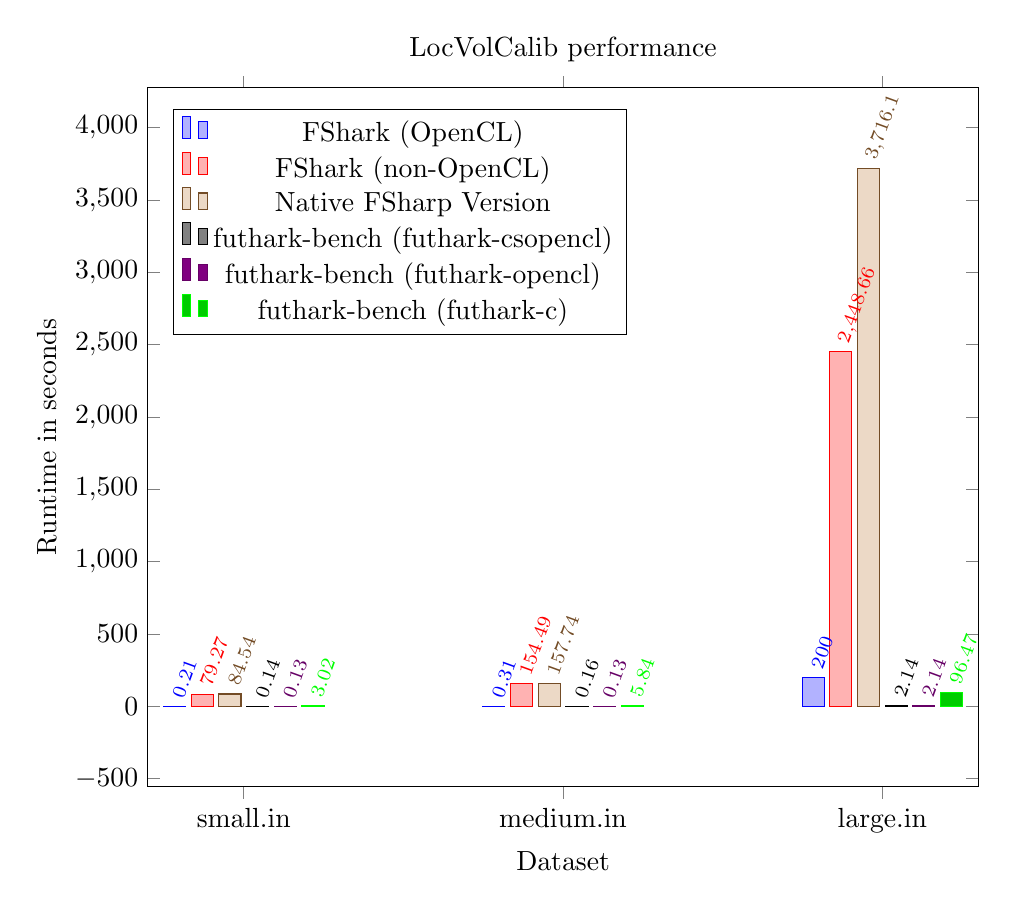
\begin{tikzpicture}
      \begin{axis}[
        title={LocVolCalib performance},
        xlabel={Dataset},
        ylabel={Runtime in seconds},
        width=1\textwidth,
        %height=0.5,
        symbolic x coords={small.in,medium.in,large.in},
        xtick=data,
        enlargelimits=0.15,
        ybar=2pt,% configures ‘bar shift’
        bar width=8pt,
        nodes near coords,
        every node near coord/.append style={rotate=70, anchor=west,font=\scriptsize},
        legend style={legend pos=north west}
      ]
      \addplot plot coordinates {(small.in, 0.21 ) (medium.in, 0.31 ) (large.in, 200.0 )};
      \addplot plot coordinates {(small.in, 79.265 ) (medium.in, 154.488 ) (large.in, 2448.660 )};
      \addplot plot coordinates {(small.in, 84.537 ) (medium.in, 157.735 ) (large.in, 3716.097 )};
      \addplot plot coordinates {(small.in, 0.14 ) (medium.in, 0.16 ) (large.in, 2.14 )};
      \addplot plot coordinates {(small.in, 0.13 ) (medium.in, 0.13 ) (large.in, 2.14 )};
      \addplot plot coordinates {(small.in, 3.02 ) (medium.in, 5.84 ) (large.in, 96.47 )};

      \legend{FShark (OpenCL), FShark (non-OpenCL), Native FSharp Version, futhark-bench (futhark-csopencl), futhark-bench (futhark-opencl), futhark-bench (futhark-c)}
      \end{axis}
    \end{tikzpicture}
    \caption{Comparison between Python and Futhark performance for simple model}
    \label{fig:line-graph}
\end{figure}

medium.in:
(Fshark opencl)invokation time was 310833 microseconds
Fshark nonopencl Average invokation time was 154 141 321 ms
Native took 900 643005 microseconds.

large.in:

fshark with opencl Memory Allocation Error
fshark sans opencl 2450 637 053 microseconds
Native took 24757 874 577 microseconds.


for all three datasets
%% master ●  futhark-bench --compiler=futhark-csopencl LocVolCalib.fut 
%%Compiling LocVolCalib.fut...
%%Results for LocVolCalib.fut:
%dataset LocVolCalib-data/small.in:   143015.70us (avg. of 10 runs; RSD: 0.02)
%dataset LocVolCalib-data/medium.in:  143581.70us (avg. of 10 runs; RSD: 0.00)
%dataset LocVolCalib-data/large.in:  1987195.20us (avg. of 10 runs; RSD: 0.00)
%%
%% master ●  futhark-bench --compiler=futhark-opencl LocVolCalib.fut 
%%Compiling LocVolCalib.fut...
%%Results for LocVolCalib.fut:
%%dataset LocVolCalib-data/small.in:   134473.30us (avg. of 10 runs; RSD: 0.02)
%%dataset LocVolCalib-data/medium.in:  134796.20us (avg. of 10 runs; RSD: 0.01)
%%dataset LocVolCalib-data/large.in:  1924412.20us (avg. of 10 runs; RSD: 0.01)

%% master ●  futhark-bench --compiler=futhark-c LocVolCalib.fut     
%%Compiling LocVolCalib.fut...
%%Results for LocVolCalib.fut:
%%dataset LocVolCalib-data/small.in:  3 020588.60us (avg. of 10 runs; RSD: 0.01)
%%dataset LocVolCalib-data/medium.in: 5 842482.00us (avg. of 10 runs; RSD: 0.01)
%%dataset LocVolCalib-data/large.in:  96 476520.00us (avg. of 10 runs; RSD: 0.00)
%%


\section*{The \texttt{nbody} benchmark}

for all three datasets


\subsection*{Specifications for benchmark}
We have run the benchmarks on a system with these attributes:
\begin{itemize}
\item CPU: 4 cores of Intel Core i5-6500 at 3.20GHz
  \begin{itemize}
  \item L1 cache: 128 KiB 
  \item L2 cache: 1024 KiB 
  \item L3 cache: 6144 KiB 
  \end{itemize}
\item GPU: GeForce GTX 970
\end{itemize}


Introduction for the two benchmarks LocVolCalib and nbody



why are they faster in general




%%% Local Variables:
%%% mode: latex
%%% TeX-master: "../thesis"
%%% End:
\chapter{Related work}

%%% Local Variables:
%%% mode: latex
%%% TeX-master: "../thesis"
%%% End:

\chapter{Conclusion and future work}

%%% Local Variables:
%%% mode: latex
%%% TeX-master: "../thesis"
%%% End:

%\bibliographystyle{ACM-Reference-Format}
%\softraggedright
\bibliographystyle{abbrv}
\bibliography{report/references.bib}

\begin{appendices}
\chapter{Implementation}
\section{Code generator}
The \csharp{} code generator is part of the Futhark project.
The Futhark implementation is located on Github:
\url{https://github.com/diku-dk/futhark}

The code generator is stored in the Futhark branch \texttt{mknu/csharp}, and
this thesis is based
on the commit \texttt{0d363e9572b1c32299332a30cadfc31d5427817a}, see\\
\url{https://github.com/diku-dk/futhark/tree/0d363e9572b1c32299332a30cadfc31d5427817a}.\\
Our implementation is located in the folder
\texttt{src/Futhark/CodeGen/Backends}.

We have been testing the code generator using the test suite located in the 
\texttt{tests} directory in Futhark's root directory.

\section{\fshark{} language and compiler}
The \fshark{} language, compiler and test suite is all located on Github:\\
\url{https://github.com/diku-dk/fshark}. It is structured as a single \fsharp{}
solution containing five \fsharp{} projects.\\
This thesis is based on the commit CCCCCCCCCCCCCCCCCCCCCC, see\\

The \fshark{} test suite can be found in the \texttt{FSharkTests} folder.\\
An executable example is shown in \texttt{Examples/Program.fs} folder.
We recommend opening and using the \fshark{} solution through an IDE such as
Jetbrains' \texttt{Rider}.

\chapter{\fshark{} standard library}
\label{appendix:soacs}
The \fshark{} standard library is available in the \fshark{} repository in the file \texttt{FSharkPrelude/FSharkPrelude.fs}.

\chapter{Program for benchmarking byte memory writes in \csharp{}}
\begin{minted}[linenos, breaklines]{csharp}
using System;
using System.Diagnostics;
using System.Runtime.InteropServices;

namespace ConsoleApplication2
{
    internal class Program
    {
        static private int TEST_SIZE = 1000000;
        
        static void UsingBuffer()
        {
            byte[] target = new byte[TEST_SIZE*sizeof(int)];
            for (int i = 0; i < TEST_SIZE; i++)
            {
                var intAsBytes = BitConverter.GetBytes(i);
                Buffer.BlockCopy(intAsBytes, 0, target, i * sizeof(int), sizeof(int)); 
            }
        }
        
        static void UsingUnsafe1()
        {
            byte[] target = new byte[TEST_SIZE*sizeof(int)];
            for (int i = 0; i < TEST_SIZE; i++)
            {
                unsafe
                {
                    fixed (byte* ptr = &target[i * sizeof(int)])
                    {
                        *(int*) ptr = i;
                    }
                }
            }
        }
        
        static void UsingUnsafe2()
        {
            byte[] target = new byte[TEST_SIZE*sizeof(int)];
            unsafe
            {
                fixed (byte* ptr = &target[0])
                {
                    for (int i = 0; i < TEST_SIZE; i++)
                    {
                        *(int*) (ptr+i*sizeof(int)) = i;
                    }
                }
            }
        }

        public static void Main(string[] args)
        {
            var TESTS = 10;
            var stopwatch = new Stopwatch();
            for (int i = 0; i < TESTS; i++)
            {
                stopwatch.Start();
                UsingBuffer();
                stopwatch.Stop();
            }

            Console.WriteLine("Safe took {0} ticks on avg.", stopwatch.ElapsedTicks / 10);

            stopwatch.Reset();

            for (int i = 0; i < TESTS; i++)
            {
                stopwatch.Start();
                UsingUnsafe1();
                stopwatch.Stop();
            }

        Console.WriteLine("Unsafe1 took {0} ticks on avg.", stopwatch.ElapsedTicks / 10);
            
            stopwatch.Reset();
            
            for (int i = 0; i < TESTS; i++)
            {
            stopwatch.Start();
            UsingUnsafe2();
            stopwatch.Stop();
            }
                
            Console.WriteLine("Unsafe2 took {0} ticks on avg.", stopwatch.ElapsedTicks / 10);

        }
    }
}
\end{minted}
{Short \csharp{} program that measures performance differences between
  various methods of writing scalars to byte arrays}
\label{fig:memoryperformancebenchmark}

\chapter{LocVolCalib benchmark written in \fshark{} and Futhark}
\label{app:fsharklocvolcalib}
To avoid adding hundreds of lines of source code to the appendices, we instead
link to the two different versions of the LocVolCalib benchmark:

The \fshark{} version is available on:\\
\url{https://github.com/diku-dk/fshark/blob/d41e5d99f37dc6c77b565ec89ee58533bb264232/FSharkTests/Benchmarks/LocVolCalib.fs}
\\
The Futhark version used is available on:\\
\url{https://github.com/diku-dk/futhark-benchmarks/blob/fd4dec357bb51d8109fed67c2e14bc5da9b20179/finpar/LocVolCalib.fut}

\chapter{nbody benchmark written in \fshark{} and Futhark}
\label{app:fsharknbody}


The \fshark{} version is available on\\
\url{https://github.com/diku-dk/fshark/blob/d41e5d99f37dc6c77b565ec89ee58533bb264232/FSharkTests/Benchmarks/Nbody.fs}

The Futhark version used is available on:\\
\url{https://github.com/diku-dk/futhark-benchmarks/blob/fd4dec357bb51d8109fed67c2e14bc5da9b20179/accelerate/nbody/nbody.fut}








\chapter{Numbers for LocVolCalib benchmarks}




\subsubsection{\fshark{} LocVolCalib with OpenCL (avg. of 10 runs)}
Runtimes for compiled \fshark{} version of LocVolCalib with OpenCL enabled.\\
\begin{tabular}{|c|c|c|}
  \hline
  \textbf{small.in} & \texttt{medium.in} & \texttt{large.in}\\ \hline \hline
187972 $\mu s$& 269265 $\mu s$ &5052080 $\mu s$\\ \hline
\end{tabular}

\subsubsection{\fshark{} LocVolCalib without OpenCL (avg. of 10 runs)}
Runtimes for compiled \fshark{} version of LocVolCalib with OpenCL disabled.\\
\begin{tabular}{|c|c|c|}
  \hline
  \textbf{small.in} & \texttt{medium.in} & \texttt{large.in}\\ \hline \hline
79265000 $\mu s$& 154488000 $\mu s$ & 2448660 $\mu s$\\ \hline
\end{tabular}

\subsubsection{Futhark benchmark version of LocVolCalib with \csharp{} OpenCL (avg. of 10 runs)}
These benchmarks are for the futhark-benchmarks version of the LocVolCalib
benchmark, compiled with the \csharp{} OpenCL code generator.
\begin{tabular}{|c|c|c|}
  \hline
  \textbf{small.in} & \texttt{medium.in} & \texttt{large.in}\\ \hline \hline
134031 $\mu s$& 134761 $\mu s$ & 1925001 $\mu s$\\ \hline
\end{tabular}

\subsubsection{Futhark benchmark version of LocVolCalib with \c{} OpenCL (avg. of 10 runs)}
These benchmarks are for the futhark-benchmarks version of the LocVolCalib
benchmark, compiled with the existing \c{} OpenCL code generator.
\begin{tabular}{|c|c|c|}
  \hline
  \textbf{small.in} & \texttt{medium.in} & \texttt{large.in}\\ \hline \hline
135190 $\mu s$& 134428 $\mu s$ & 1911079 $\mu s$\\ \hline
\end{tabular}

\end{appendices}






%%% Local Variables:
%%% mode: latex
%%% TeX-master: "../thesis"
%%% End:
\end{document}


%%% Local Variables:
%%% coding: utf-8
%%% mode: latex
%%% TeX-command-extra-options: "-shell-escape"
%%% End:
